%! Compiler = pdflatex --shell-escape

\documentclass[12pt, listof=totoc, bibliography=totoc, parskip=full, numbers=noenddot]{scrreprt}
\setcounter{secnumdepth}{\subsubsectionnumdepth}

\newcommand{\mytitle}{ADDING A THIRD NORMAL TO CLUBB}
\newcommand{\myauthor}{Sven Bergmann}

\RedeclareSectionCommand[beforeskip=0pt]{chapter}

\usepackage[top=1in, bottom=1in, left=1in, right=1in, letterpaper]{geometry}

\usepackage{setspace}
\setdisplayskipstretch{}

\usepackage{bm}
\usepackage{hyperref}
\usepackage[standard, hyperref]{ntheorem}
\usepackage{amsmath}
\usepackage{amsfonts}
\numberwithin{equation}{chapter}
\numberwithin{equation}{section}
\usepackage[acronym, toc]{glossaries}
\setglossarystyle{list}
\newglossary[slg]{symbolslist}{syi}{syg}{\normalfont{LIST OF SYMBOLS}}

\newglossaryentry{w_prime}{
    name={$w'$},
description={Standardized upward wind ($w' = w - \overline{w}$)},
type=symbolslist
}

\newglossaryentry{r_t_prime}{
name={$r_t'$},
description={Standardized total water mixing ratio ($r_t' = r_t - \overline{r_t}$)},
type=symbolslist
}

\newglossaryentry{theta_l_prime}{
name={$\theta_l'$},
description={Standardized liquid water potential temperature ($\theta_l' = \theta_l - \overline{\theta_l}$)},
type=symbolslist
}

\newglossaryentry{theta_l_prime_tilde}{
name={$\tilde{\theta}_l'$},
description={Normalized liquid water potential temperature (see \cref{eq:theta_l_prime_tilde}},
type=symbolslist
}

\newglossaryentry{r_t_prime_tilde}{
name={$\tilde{r}_t'$},
description={Normalized total water mixing ratio (see \cref{eq:r_t_prime_tilde}},
type=symbolslist
}

\renewcommand*{\acronymname}{\normalfont{LIST OF ACRONYMS}}

\newacronym{CLUBB}{CLUBB}{Cloud Layers Unified By Binormals}

\newacronym{pdf}{pdf}{probability density function}

\newacronym{SILHS}{SILHS}{Subgrid Importance Latin Hypercube Sampler}

\newacronym{cas}{cas}{computer algebra system}

\newacronym{pde}{pde}{partial differential equation}

\newacronym{lhs}{lhs}{left hand side}

\newacronym{rhs}{rhs}{right hand side}
\makeglossaries
\usepackage{graphicx}

\usepackage[newfloat, outputdir=../auxil]{minted}
\newminted{python}{
    autogobble,
    frame=single,
    fontsize=\footnotesize
}

%\usepackage{pgfplots}
%\pgfplotsset{compat=newest}
%\usepgfplotslibrary{external}
%\tikzexternalize

\usepackage{csquotes}
\usepackage[nameinlink,noabbrev]{cleveref}


\newcommand{\wptwo}{ \overline{w'^2} }
\newcommand{\thlptwo}{ \overline{\theta_l'^2} }
\newcommand{\rtptwo}{ \overline{r_t'^2} }
\newcommand{\wpthlp}{ \overline{w' \theta_l'} }
\newcommand{\wprtp}{ \overline{w' r_t'} }
\newcommand{\rtpthlp}{ \overline{r_t' \theta_l'} }
\newcommand{\wptwothlp}{ \overline{w'^2 \theta_l'} }
\newcommand{\wptwortp}{ \overline{w'^2 r_t'} }
\newcommand{\wpthlptwo}{ \overline{w' \theta_l'^2} }
\newcommand{\wprtptwo}{ \overline{w' r_t'^2} }
\newcommand{\wprtpthlp}{ \overline{w' r_t' \theta_l'} }
\newcommand{\wpthree}{ \overline{w'^3} }
\newcommand{\thlpthree}{ \overline{\theta_l'^3} }
\newcommand{\rtpthree}{ \overline{r_t'^3} }
\newcommand{\wpfour}{ \overline{w'^4} }

\newcommand{\tsw}{{\tilde{\sigma}_w}}
\newcommand{\tswfact}{\left( 1 - \tilde{\sigma}_w^2 \right)}

\begin{document}

    \doublespacing

    \setcounter{page}{1}
    \thispagestyle{empty}

    \begin{center}
{\Large ADDING A THIRD GAUSSIAN TO CLUBB}
    \\
    \vspace{0.6\baselineskip}
    by\\
    Sven Bergmann\\
    \vspace{2in}
    A Dissertation Submitted in\\
    Partial Fulfillment of the\\
    Requirements for the Degree of\\
    \vspace{0.5in}
    Master of Science\\
    in Mathematics\\
    \vspace{0.5in}
    at\\
    The University of Wisconsin--Milwaukee\\
    Mai 2023\\
\end{center}

    \newpage
    \clearpage
    \pagestyle{plain}
    \pagenumbering{roman}
    \setcounter{page}{2}

    \begin{center}
    ABSTRACT
    \\
    \singlespacing
    ADDING A THIRD GAUSSIAN TO CLUBB\\
    \doublespacing
    by\\
    Sven Bergmann\\
    \singlespacing
    The University of Wisconsin--Milwaukee, 2024\\
    Under the Supervision of Professor Vince Larson
\end{center}

The \gls{CLUBB} model uses the sum of two Normal \glspl{pdf} to describe a grid layer of the atmosphere.
To do that, \gls{CLUBB} uses a large set of \glspl{pde}.
For advancing in time, there are some values for higher order moments needed, e.g. for the upward wind, and the liquid water potential temperature, which are being described by backing out the \gls{pdf} parameters from some equations for lower order moments and then compute the higher order moments in terms of the lower order ones.
Going through this process, \gls{CLUBB} can then close the equations.
Since \gls{CLUBB} is only using two added up Normal \glspl{pdf}, it cannot really model every possible shape of the grid layers.
Therefore the idea came in mind to add a third Normal \glspl{pdf} right in the middle of the already existing Normal \glspl{pdf} without making the equations too complicated and also numerically still realizable.
This document then describes all formulas, inputs and outputs and also tries to take a closer look at some asymptotic behaviors.


    \newpage
    \hspace{0pt}
    \vfill
    \begin{center}
        Type dedication here.
    \end{center}
    \vfill


    \singlespacing
    \renewcommand*\contentsname{\centering\normalfont{TABLE OF CONTENTS}}
    \tableofcontents
    \newpage

    \doublespacing

    \renewcommand*\listfigurename{\centering\normalfont{LIST OF FIGURES}}
    \listoffigures
    \newpage


    \renewcommand*\listtablename{\centering\normalfont{LIST OF TABLES}}
    \listoftables
    \newpage

    \renewcommand*\listlistingname{\centering\normalfont{LIST OF LISTINGS}}
    \listoflistings
    \newpage

    \printglossary[type=\acronymtype, title={\centering\normalfont{LIST OF ACRONYMS}}]
    \newpage

    \printglossary[type=symbolslist, title={\centering\normalfont{LIST OF SYMBOLS}}]
    \newpage

    \thispagestyle{plain}

%    \addcontentsline{toc}{chapter}{\centering\normalfont{ACKNOLEDGEMENTS}}
\chapter*{\centering\normalfont{ACKNOLEDGEMENTS}}\label{ch:acknowledgements}

The following work is based on a the papers
\citetitle{larson2005using} by \citeauthor{larson2005using} and
\citetitle{larson2022clubbsilhs} by \citeauthor{larson2022clubbsilhs}.
%    \newpage

    \pagenumbering{arabic}

    \chapter{Introduction}\label{ch:introduction}

The \gls{CLUBB} model is a powerful tool used to simulate atmospheric behavior within climate models.
This document explores an extension to the current \gls{CLUBB} framework.
Currently, \gls{CLUBB} utilizes the sum of two normal \glspl{pdf}
to represent a single atmospheric grid layer.
While effective,
this approach limits the model's ability to capture the full spectrum of potential cloud layer shapes.
This work proposes an innovative solution:
incorporating a third normal \gls{pdf} into the \gls{CLUBB} framework.
This addition aims to enhance the model's representational capabilities
while maintaining computational efficiency and numerical stability.
To achieve this, the document dives into the details of the proposed method.

We begin by outlining the core problem we aim to address (\cref{ch:problem})
by starting with the motivation,
proceeding with a short explanation on how to close turbulence \glspl{pde}
(\cref{sec:closing-turbulence-pdes-by-integration-over-a-pdf})
and explaining how we derive the transformation from the formulas
given by the paper~\citetitle{larson2005using}
by~\citeauthor{larson2005using}~[\citeyear{larson2005using}]
(\cref{sec:derivation-of-trinormal-closures-by-transformation-of-binormal-closures}).
After that, we define the goal of this thesis (\cref{sec:goal-of-this-thesis}),
talk about the inputs and outputs (\cref{sec:inputs-and-outputs-of-the-verification-procedure})
and provide steps for checking those formulas (\cref{sec:steps-for-checking-the-formulas}).

Following this motivational chapter,
we establish a foundation with clear definitions of the relevant concepts,
including normal distributions and the thermodynamic scalars
crucial for atmospheric modeling (\cref{ch:definitions}).

\Cref{ch:formulas-that-define-the-shape-of-the-pdf-and-moments-in-terms-of-pdf-parameters} forms the heart of this work,
presenting the actual formulas associated with the extended \gls{CLUBB} model.
This chapter details the introduction of the third normal \gls{pdf} (\cref{sec:definition-of-the-trinormal-distribution-p_tmg})
and the derivation of key moments within the model
(\cref{sec:a-list-of-lower-order-moments-expressed-in-terms-of-pdf-parameters} -
\cref{sec:solving-for-pdf-parameters-by-using-the-moment-terms}).
Additionally,
\cref{sec:approximation-of-scalar-skewnesses} proposes an approximation
to account for the scalar skewness,
while \cref{sec:formulating-closure-relationships-for-higher-order-moments-in-terms-of-lower-order-moments}
introduces analytic closure relations
for higher-order moments based on the newly formed mixture of three normal distributions.

For ensuring some limiting behaviour,
\cref{ch:asymptotics} investigates the asymptotics of the extended model.

Finally, to handle the mathematical integrations required by the model,
\cref{ch:integration-using-sympy} explores both,
exact parametric and numerical integration techniques of verifying the integrals,
utilizing the SymPy library (\cref{sec:analytic-integration} \& \cref{sec:numeric-integration}).

Having talked about the trinormal representation within the \gls{CLUBB} model,
\cref{ch:summary} provides a concise recap of the key findings.
This summary serves as a comprehensive overview of the essential concepts
explored throughout this thesis.

The document concludes with an outlook in \cref{ch:outlook},
outlining potential future directions for research
and exploration based on the findings presented here.

    \chapter{Problem}\label{ch:problem}

\section{Motivation}\label{sec:motivation}

As being said in the \cref{ch:introduction},
we try to describe more possible shapes with adding a third \gls{pdf}.
To illustrate that, we plot some of the shapes which are now possible but were not possible before.
To be able to draw those plots, we are just using two variables, $w$, the upward wind,
and $\theta_l$, the liquid water potential temperature.
To show how the binormal model handles strong winds,
let us consider a scenario with a strong updraft at $w_1$, as well as a strong downdraft at $w_2$.
The way the current binormal model would handle this could look like \cref{fig:plot1}.
\begin{figure}[!htb]
    \centering
    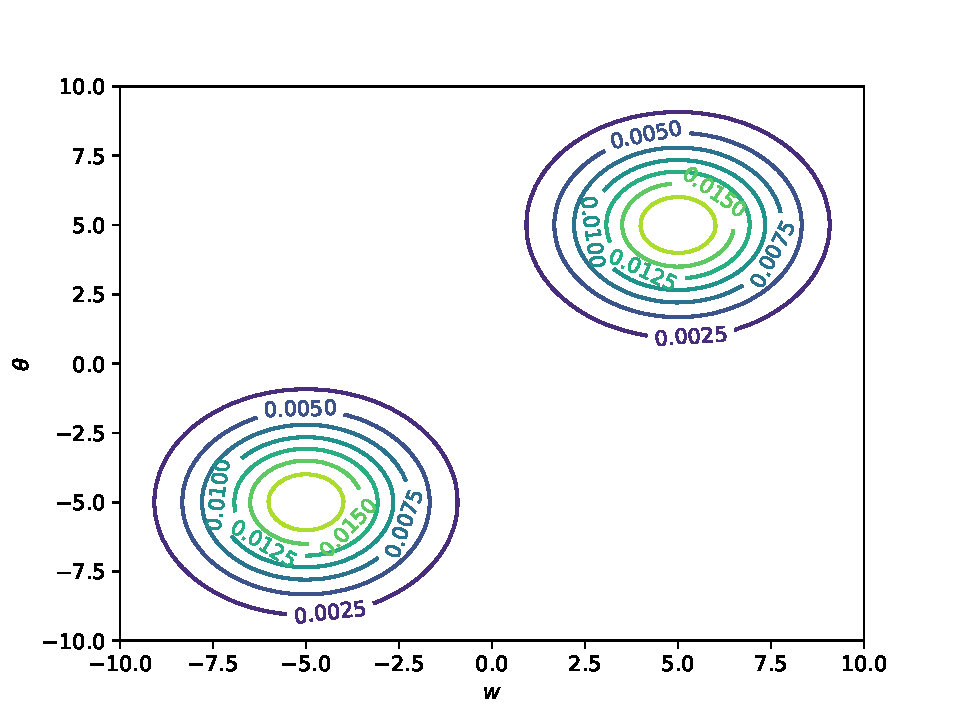
\includegraphics[width=.48\textwidth]{include/figures/plot1}
    \caption{Binormal plot for two strong up-/downdrafts}
    \label{fig:plot1}
    $w_1 = 5$, $w_2 = -5$, $\theta_{l1} = 5$, $\theta_{l2} = -5$,
    $\alpha = 0.5$, $\sigma_w = 2$, $\sigma_{\theta_{l1}} = 2$, $\sigma_{\theta_{l1}} = 2$.
\end{figure}
However, this binormal distribution (\cref{fig:plot1}) does not accurately reflect reality.
In nature, we would not expect such a sharp jump between the strong up- and downdrafts at $w_1$ and $w_2$.
There would most likely be some weaker drafts present in-between.
The current binormal model can attempt to capture this smoother transition
by simply increasing the standard deviations of both wind,
and liquid water potential temperature distributions.
This results in a broader distribution with a connection between the two peaks,
as shown in \cref{fig:plot2}.
\begin{figure}[!htb]
    \centering
    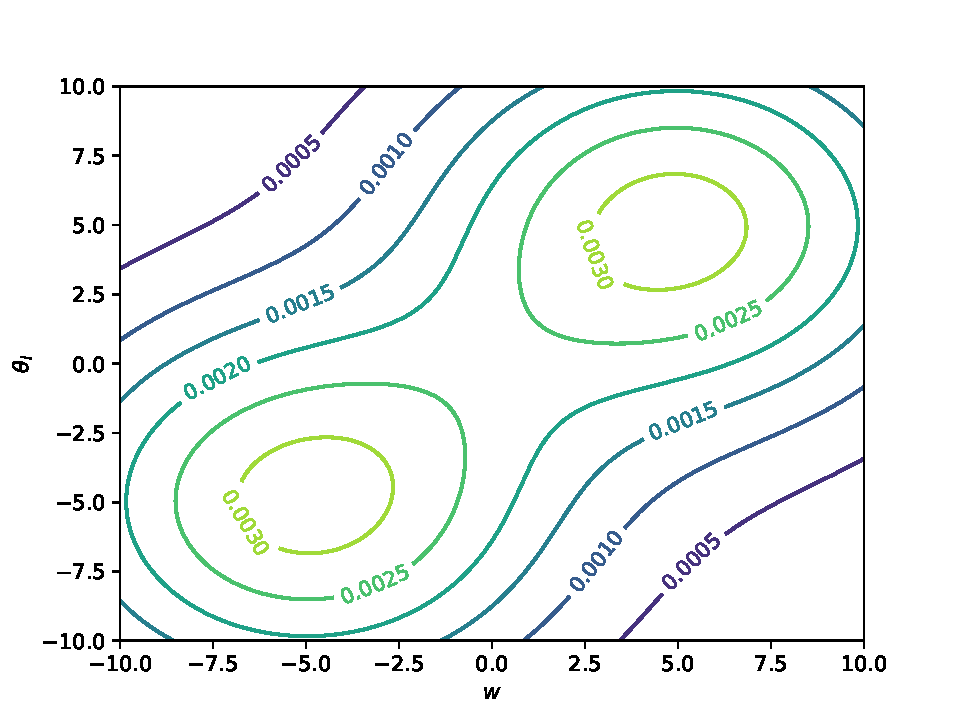
\includegraphics[width=.5\textwidth]{include/figures/plot2}
    \caption{Binormal plot for two strong up-/downdrafts with increased standard deviations}
    \label{fig:plot2}
    $w_1 = 5$, $w_2 = -5$, $\theta_{l1} = 5$, $\theta_{l2} = -5$,
    $\alpha = 0.5$, $\sigma_w = 5$, $\sigma_{\theta_{l1}} = 5$, $\sigma_{\theta_{l1}} = 5$.
\end{figure}
Seeing \cref{fig:plot2},
the issue with having some values in the middle is slightly fixed
but the general width of the normals was increased, too.
Since \gls{CLUBB} also has the simplification
that there is no correlation between $w$ and $\theta_l$,
and $w$ and $r_t$ -- obviously -- one cannot just increase it.
Therefore, the idea is to add this third normal distribution,
which actually has correlation between all three variables
and especially in the bivariate case, between $w$ and $\theta_l$.
\Cref{fig:plot2} would then change to \cref{fig:plot3}.
\begin{figure}[!htb]
    \centering
    \begin{tabular}{cc}
        \multicolumn{1}{c}{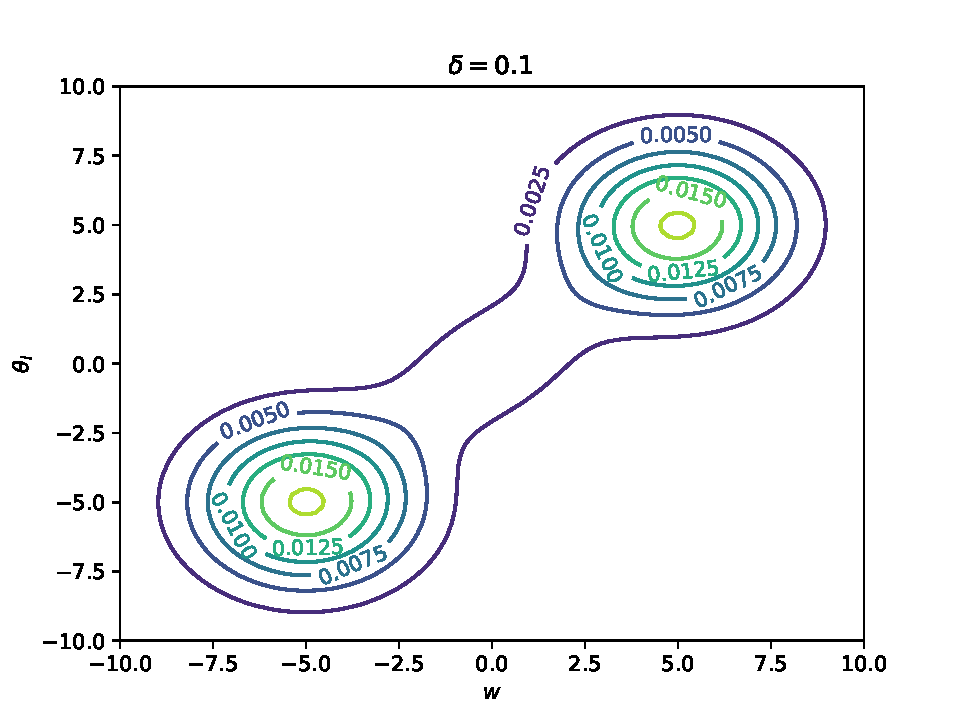
\includegraphics[width=0.48\textwidth]{include/figures/plot3_1}} &
        \multicolumn{1}{c}{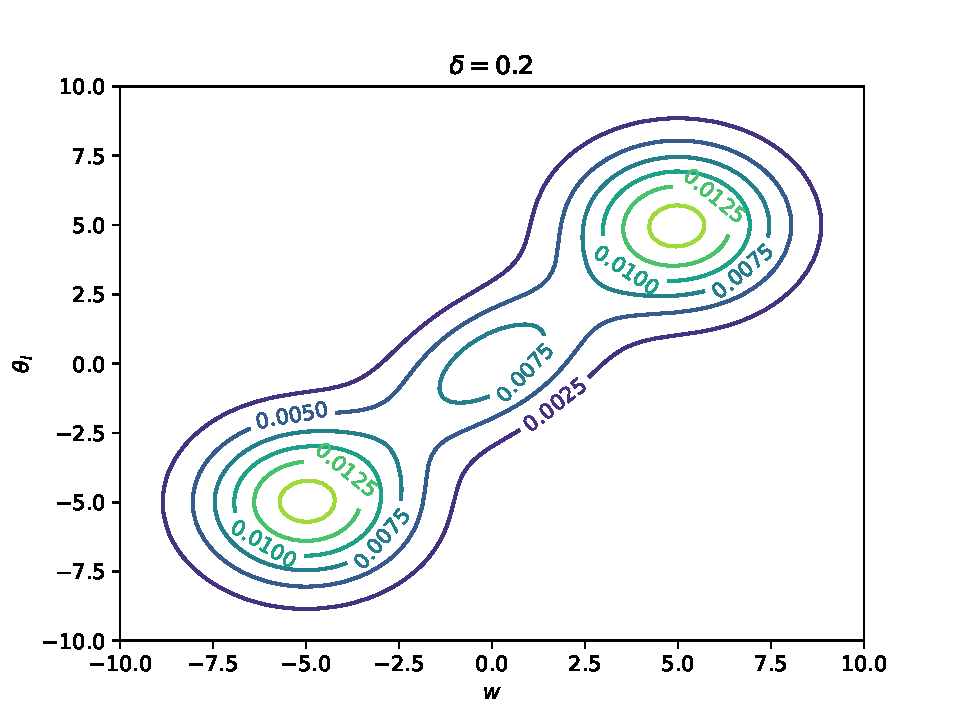
\includegraphics[width=0.48\textwidth]{include/figures/plot3_2}} \\
        \multicolumn{1}{c}{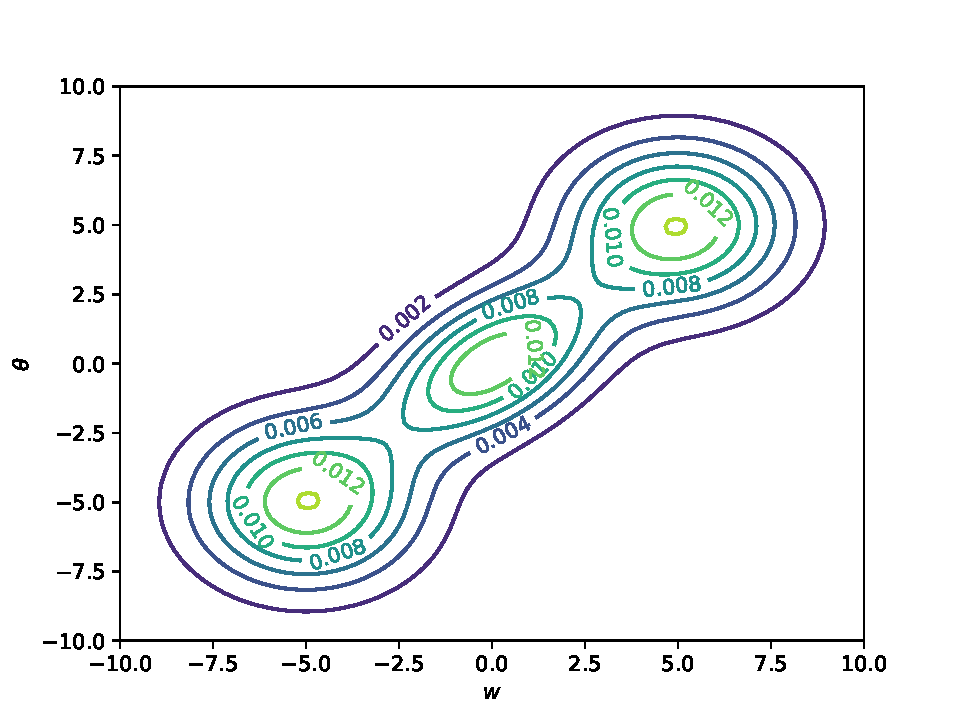
\includegraphics[width=0.48\textwidth]{include/figures/plot3_3}} &
        \multicolumn{1}{c}{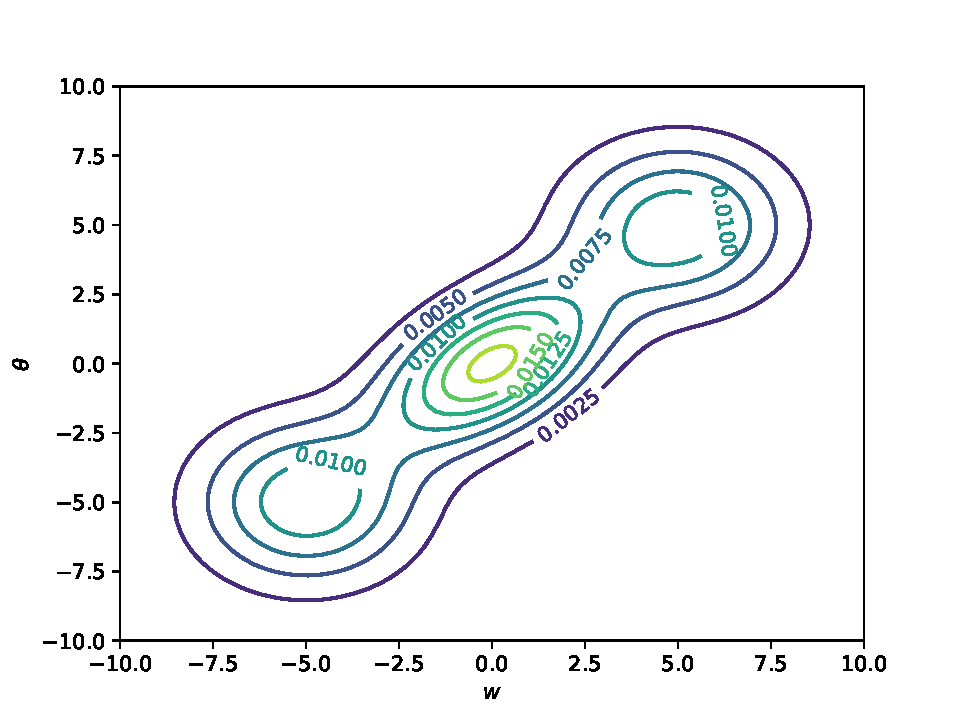
\includegraphics[width=0.48\textwidth]{include/figures/plot3_4}} \\
    \end{tabular}
    \caption{Trinormal plot for two strong up-/downdrafts with varying $\delta$}
    \label{fig:plot3}
    $w_1 = 5$, $w_2 = -5$, $\theta_{l1} = 5$, $\theta_{l2} = -5$,
    $\alpha = 0.5$, $\sigma_w = 2$, $\sigma_{\theta_{l1}} = 2$,  $\sigma_{\theta_{l2}} = 2$,
    $\sigma_{w3} = 2$, $\sigma_{3\theta_l} = 2$, $\rho_{w\theta_l} = 0.5$.
\end{figure}
Now, one can easily model something like the described shape,
as illustrated in \cref{fig:plot3}.
Also, some other (maybe weird) shapes are now possible,
just like the one in \cref{fig:plot4}.
\begin{figure}[!htb]
    \centering
    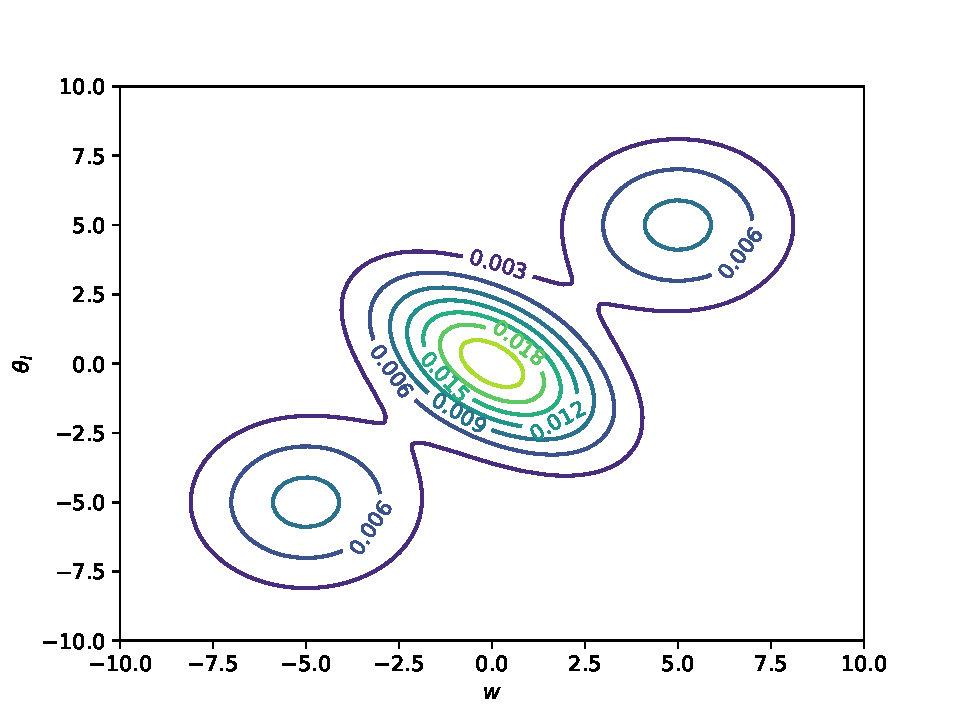
\includegraphics[width=.5\textwidth]{include/figures/plot4}
    \caption{Trinormal plot for two strong up-/downdrafts with a third peak in the middle}
    \label{fig:plot4}
    $w_1 = 5$, $w_2 = -5$, $\theta_{l1} = 5$, $\theta_{l2} = -5$,
    $\alpha = 0.5$, $\delta=0.5$, $\sigma_w = 2$, $\sigma_{\theta_{l1}} = 2$,
    $\sigma_{\theta_{l2}} = 2$, $\sigma_{w3} = 2$, $\sigma_{\theta_l 3} = 2$,
    $\rho_{w\theta_l} = 0.5$.
\end{figure}


\section{Closing pdes}\label{sec:closing_pdes}

The \gls{CLUBB} model relies on a set of \glspl{pde} to represent atmospheric processes.
These equations require closure,
implying the expression of all terms solely in terms of known quantities.
This closure process often involves integrals,
and verifying their analytical solutions ensures the model's mathematical integrity.
For instance, consider the following prognostic {\gls{pde}\autocite[p. 21]{larson2022clubbsilhs}}:
\begin{align*}
    \frac{\partial \overline{w'r_t'}}{\partial t}
    &= -\overline{w}\frac{\partial \overline{w'r_t'}}{\partial z}
    - \frac{1}{\rho_s} \frac{\partial \rho_s \overline{w'^2 r_t'}}{\partial z}
    - \overline{w'^2} \frac{\partial \overline{r_t'}}{\partial z}
    - \overline{w'r_t'} \frac{\partial \overline{w}}{\partial z}
    + \ldots
\end{align*}
While the details of initial and boundary conditions are essential
for formally closing the prognostic equations in \gls{CLUBB} (omitted for brevity),
this section emphasizes the importance of efficiently calculating moments
on the \gls{rhs} of these equations.
That is because the model steps forward in time
and therefore needs the repeated calculation of moments
for each unclosed prognostic equation at every time step.
Those already expensive computational steps need to use mathematically simpler moment representations
of e.g. $\overline{w'^2 r_t'}$,
even if they introduce slight limitations
in capturing the full variability of the underlying atmospheric state.
Our focus here is on achieving closure for higher-order moments,
such as the third order moment $\overline{w'^2 r_t'}$ and others like it.
This closure is achieved by expressing these higher-order moments
in terms of readily calculable lower-order moments.
This approach uses the relationships between moments within a normal distribution,
enabling efficient model updates during the time-stepping process.

\section{Transformation of the equations}\label{sec:transformationequations}

Having established the definition of the sum of normal distributions in \cref{sec:def_trinormal}
to enhance mathematical tractability,
we now delve into the transformation of equations from the existing binormal representation
used in CLUBB-SILHS\autocite{larson2022clubbsilhs} to a trinormal one.
While the formulas for the binormal case are well-defined (see~CLUBB-SILHS\autocite{larson2022clubbsilhs}),
the simplicity of the means and standard deviations employed in the trinormal representation suggests
the existence of a specific transformation that holds true.
This chapter will demonstrate that the following transformations,
denoted by the subscript \enquote{dGn} for the binormal case,
successfully achieve this conversion.
\begin{align}
    \overline{w'^2} \frac{1 - \delta\lambda_w}{1 - \delta}
    &= \overline{w'^2}_{dGn}, \label{eq:w_prime_2_transform}
\end{align}
\begin{align}
    \overline{w'^3} \frac{1}{1 - \delta}
    &= \overline{w'^3}_{dGn}, \label{eq:w_prime_3_transform}
\end{align}
\begin{align}
    \frac{\overline{w'^3}}{\overline{w'^2}^{3/2}} \frac{(1 - \delta)^{1/2}}{(1 - \lambda_w\delta)^{3/2}}
    &= \frac{\overline{w'^3}_{dGn}}{\overline{w'^2}_{dGn}^{3/2}}, \label{eq:w_prime_3_div_w_prime_2_transform}
\end{align}
\begin{align}
    \overline{\theta_l'^2} \frac{1 - \delta\lambda_\theta}{1 - \delta}
    &= \overline{\theta_l'^2}_{dGn}, \label{eq:theta_l_prime_transform}
\end{align}
\begin{align}
    \overline{w'\theta_l'} \frac{1 - \delta\lambda_{w\theta}}{1 - \delta}
    &= \overline{w'\theta_l'}_{dGn}, \label{eq:w_prime_theta_l_prime_transform}
\end{align}
\begin{align}
    \left(\overline{w'^4} - 3\delta\lambda_w^2 \left(\overline{w'^2}\right)^2\right) \frac{1}{1 - \delta}
    &= \overline{w'^4}_{dGn} \label{eq:w_prime_4_transform}
\end{align}
\begin{align}
    \left(\frac{\overline{w'^4}}{(\overline{w'^2})^2} - 3\delta\lambda_w^2 \right) \frac{1 - \delta}{(1 - \lambda_w\delta)^2}
    &= \frac{\overline{w'^4}_{dGn}}{(\overline{w'^2}_{dGn})^2} \label{eq:w_prime_4_div_w_prime_2_transform}
\end{align}
To get a sense of what those transformations mean and why they should work,
we pick e.g. \cref{eq:w_prime_2_transform}.
If we substitute in the already defined formula for $\lambda_w$ (\cref{eq:lambda}), we get
\begin{align}
    \overline{w'^2} (1 - \delta\frac{\sigma_{w 3}^2}{\wptwo})
    &= (1 - \delta)\overline{w'^2}_{dGn} \nonumber\\
    \overline{w'^2} - \delta\sigma_{w 3}^2
    &= (1 - \delta)\overline{w'^2}_{dGn} \nonumber\\
    \overline{w'^2}
    &= \overline{w'^2}_{dGn} - \delta\overline{w'^2}_{dGn} + \delta\sigma_{w 3}^2 \nonumber\\
    \overline{w'^2}
    &= \overline{w'^2}_{dGn} - \delta\left(\overline{w'^2}_{dGn} - \sigma_{w 3}^2\right).
\end{align}
Our analysis reveals a key relationship between the parameter $\delta$
and the overall variance (often referred to as \enquote{width}) of the trinormal distribution.
As the value of $\delta$ approaches 1 (but strictly remains less than 1),
the standard deviation of the third normal distribution
has a progressively stronger influence on the overall variance of the combined distribution.
This intuitively makes sense because a larger weight assigned to the third normal distribution through $\delta$
will contribute more significantly to the spread of the combined \gls{pdf}.

Also, if we look at \cref{eq:w_prime_3_transform}, we see that there is no more $\lambda_w$ present.
It makes sense graphically, that as $\delta$ grows,
which means that the normal \gls{pdf} in the middle is growing,
the overall skewness of all three normals has to change also,
depending on the value of $\sigma_{w 3}$.
We can see this, as well as the relationship between the variance in \cref{tab:1dplotbitri}.
\begin{table}[!htb]
    \centering
    \begin{tabularx}{\textwidth}{l|@{}Y@{}@{}Y@{}@{}Y@{}}
        \diagbox{$\sigma_{w 3}$}{$\delta$} & 0.1 & 0.5 & 0.9 \\
        \toprule
        0.5 & 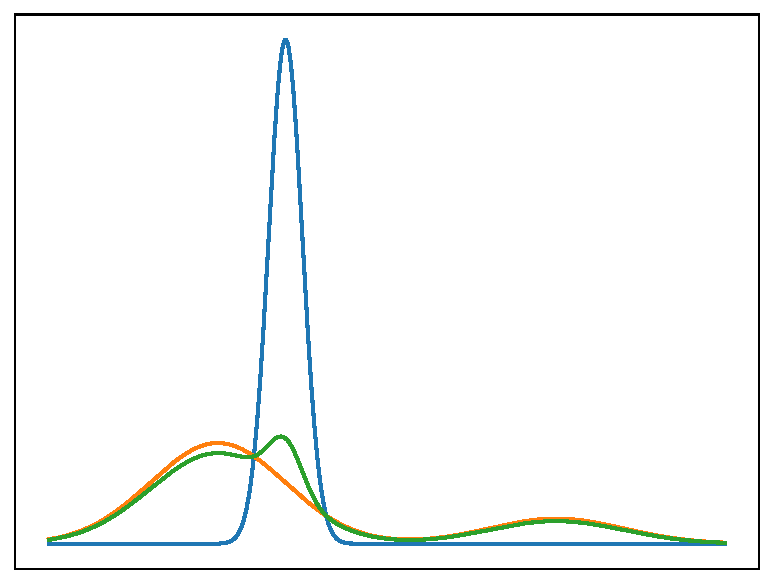
\includegraphics[width = .29\textwidth]{include/figures/1dplotslw5_delta1}
        & 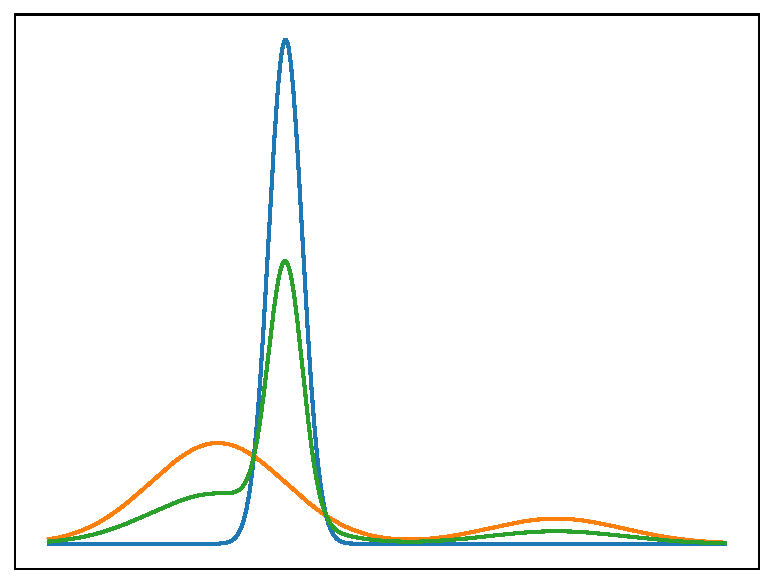
\includegraphics[width = .29\textwidth]{include/figures/1dplotslw5_delta5}
        & 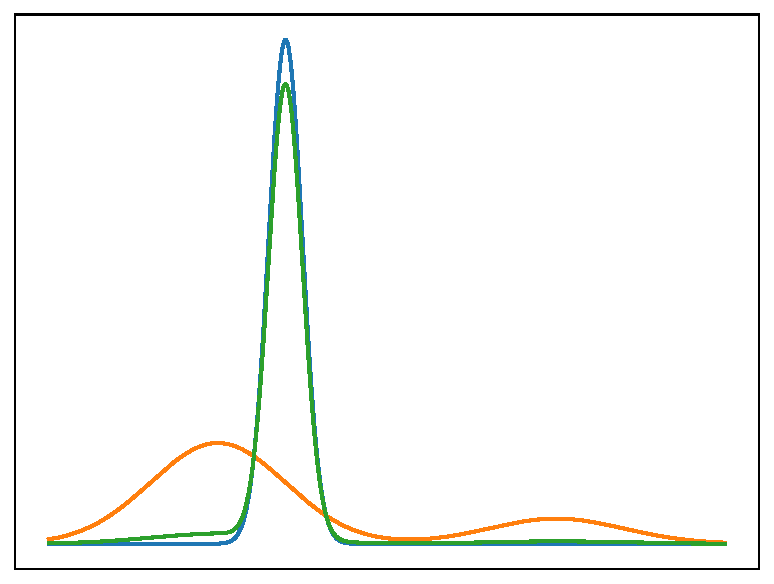
\includegraphics[width = .29\textwidth]{include/figures/1dplotslw5_delta9} \\
        \midrule
        4 & 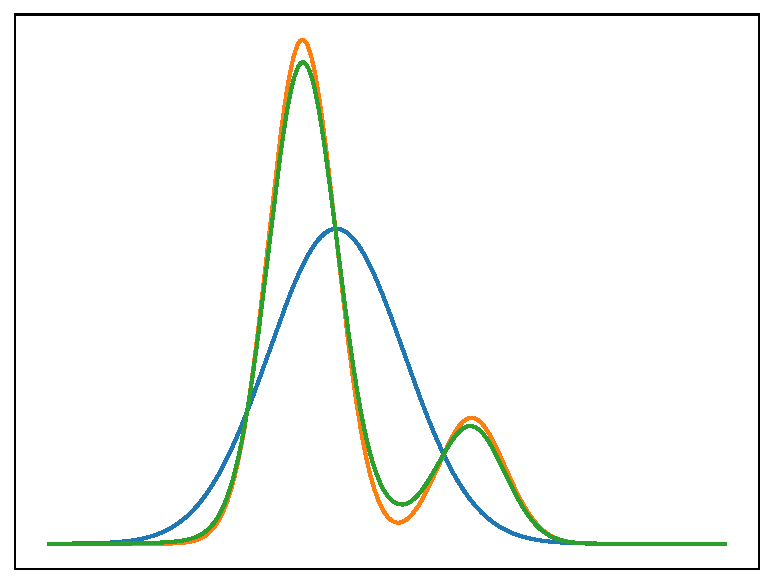
\includegraphics[width = .29\textwidth]{include/figures/1dplotslw40_delta1}
        & 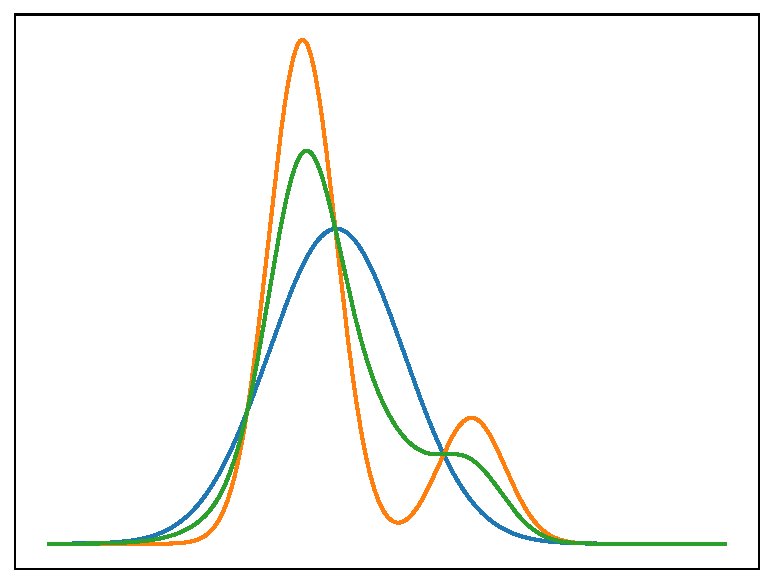
\includegraphics[width = .29\textwidth]{include/figures/1dplotslw40_delta5}
        & 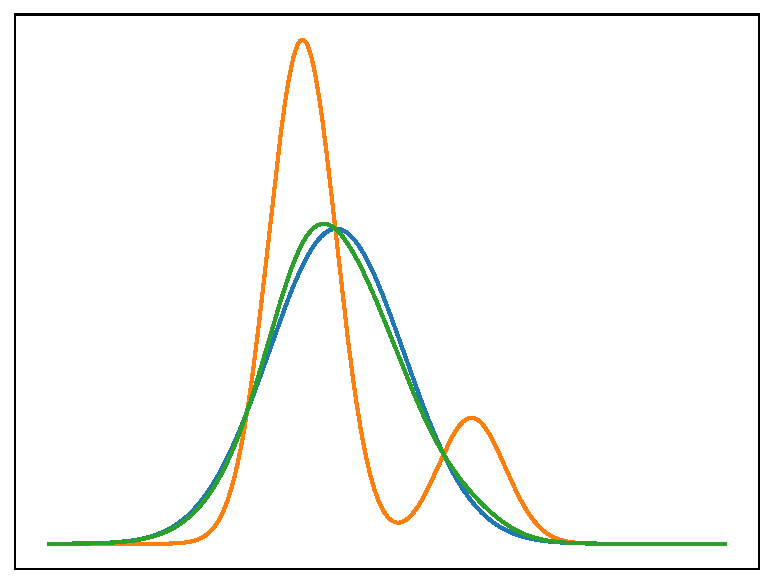
\includegraphics[width = .29\textwidth]{include/figures/1dplotslw40_delta9} \\
        \midrule
        8 & 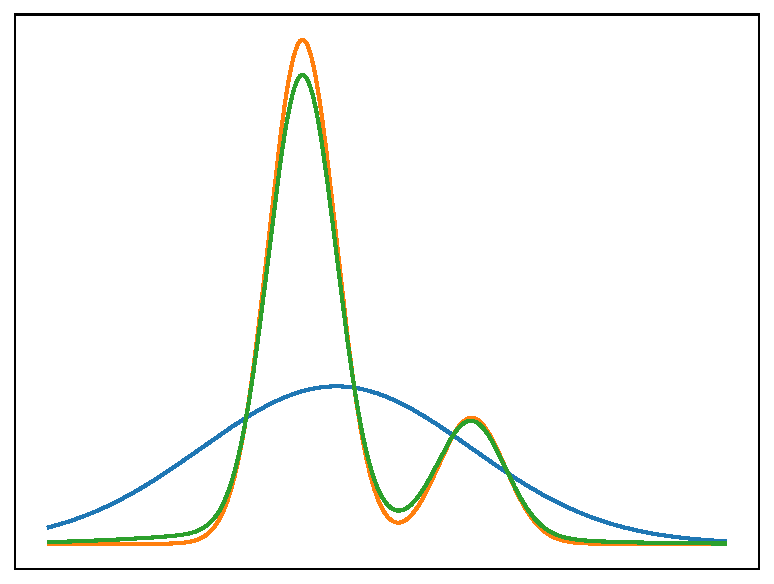
\includegraphics[width = .29\textwidth]{include/figures/1dplotslw80_delta1}
        & 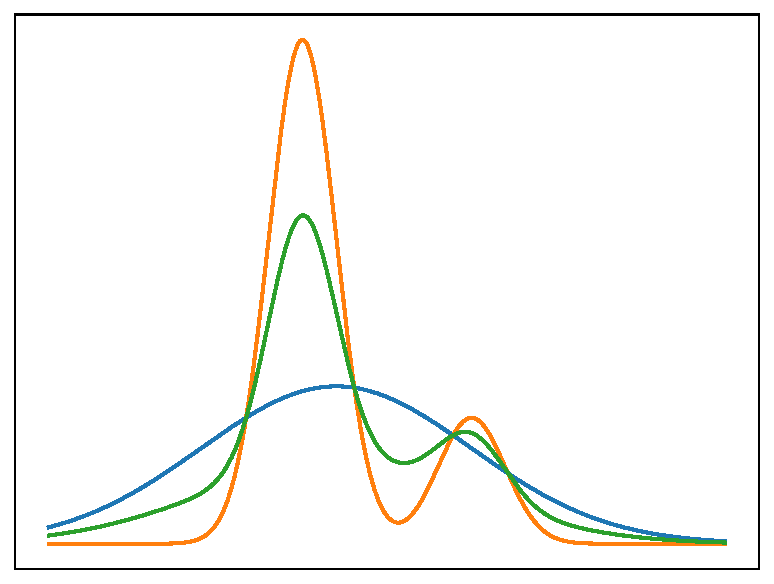
\includegraphics[width = .29\textwidth]{include/figures/1dplotslw80_delta5}
        & 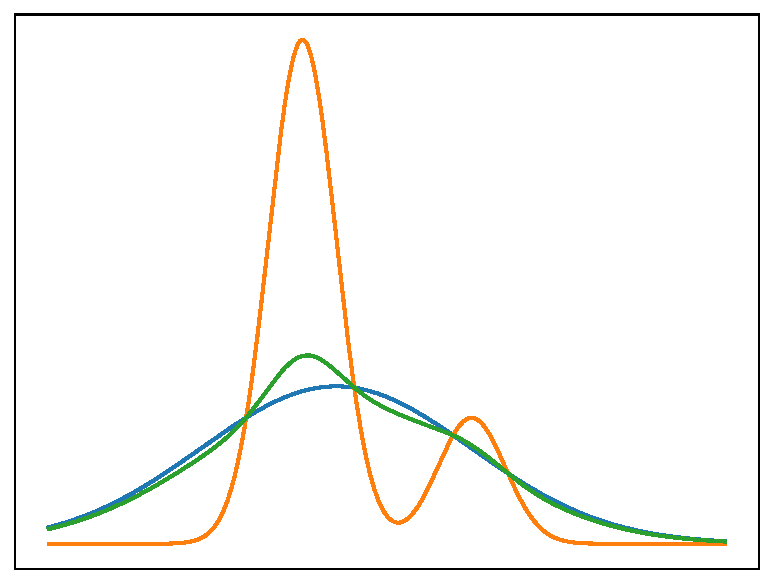
\includegraphics[width = .29\textwidth]{include/figures/1dplotslw80_delta9} \\
        \midrule
        10 & 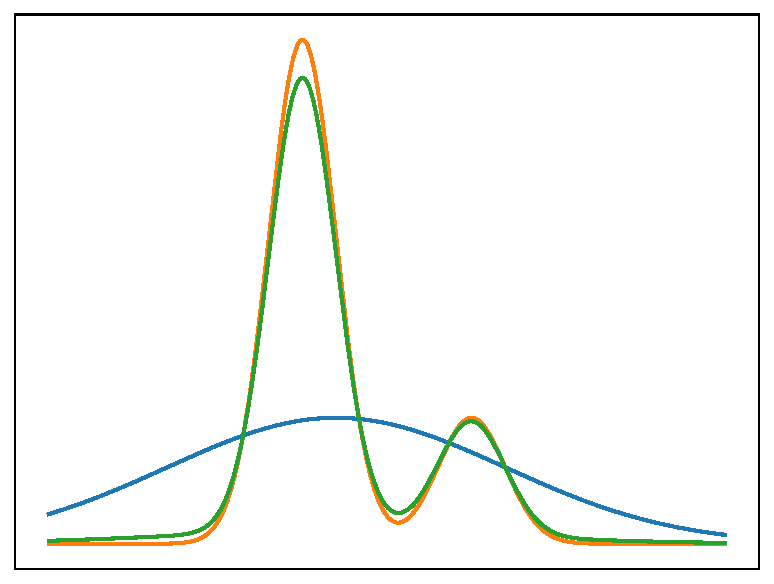
\includegraphics[width = .29\textwidth]{include/figures/1dplotslw100_delta1}
        & 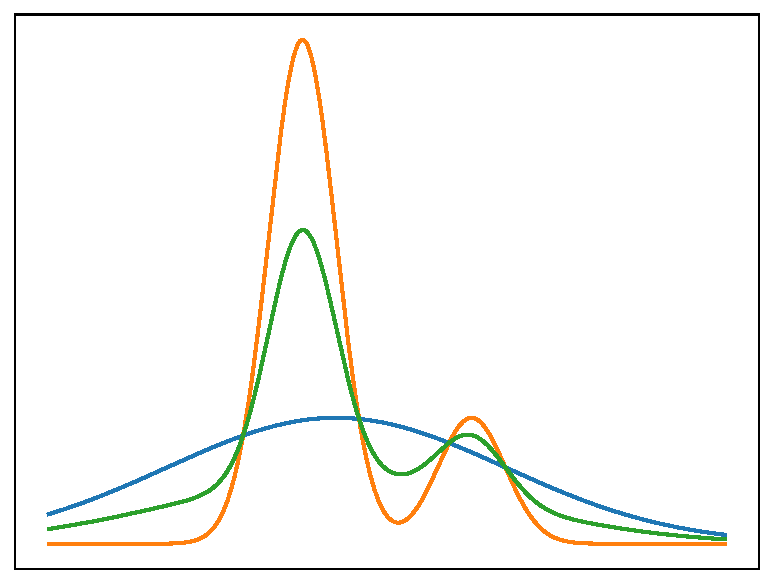
\includegraphics[width = .29\textwidth]{include/figures/1dplotslw100_delta5}
        & 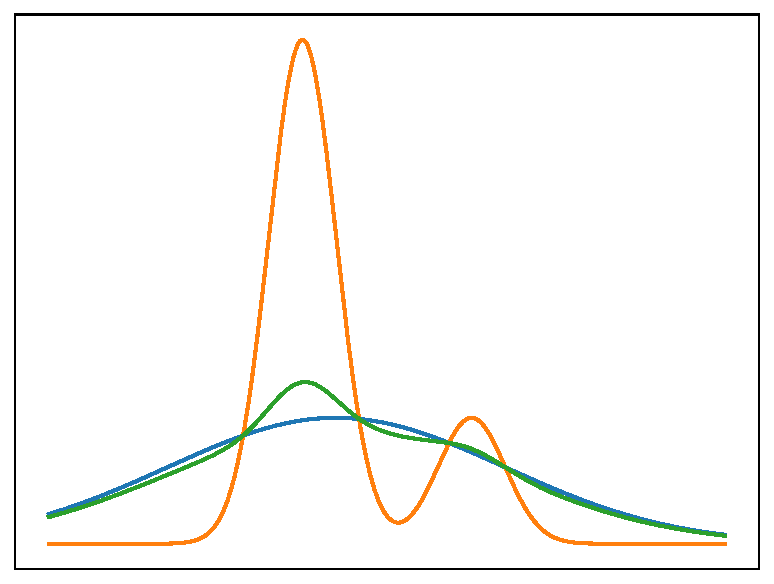
\includegraphics[width = .29\textwidth]{include/figures/1dplotslw100_delta9}
    \end{tabularx}
    \caption{1D Plots for different $\delta$ and $\sigma_{w3}$}
    $w_1 = 5$, $w_2 = -5$, $\alpha = 0.2$, $\sigma_w = 2$.
    The blue plot represents the third normal,
    the orange/red one represents the binormal,
    and the green one represents the mixture.
    The $x$ and $y$ labels and ticks are omitted for clarity.
    \label{tab:1dplotbitri}
\end{table}
\Cref{tab:1dplotbitri} offers a visual representation of how the parameter $\delta$ influences
the shape of the trinormal distribution.
Each plot illustrates \glspl{pdf} for different combinations of $\sigma_{w 3}$
(standard deviation of the third normal distribution) and $\delta$.
The row values in the table correspond to $\sigma_{w 3}$,
while the column values represent $\delta$.
We can observe two key trends within these plots:
\begin{enumerate}
    \item \emph{Influence of $\sigma_{w3}$:}
    As expected, varying $\sigma_{w3}$ primarily affects the \enquote{width}
    or overall variance of the combined distribution.
    When $\sigma_{w3}$ is larger than the width of the original binormal sum (orange/red line),
    choosing a larger $\delta$ allows the overall variance to increase significantly,
    as predicted by \cref{eq:w_prime_2_transform}.

    \item \emph{Decreasing skewness with increasing $\delta$:}
    The plots also reveal a distinct relationship between $\delta$
    and the skewness of the resulting distribution.
    As $\delta$ increases,
    the skewness of the combined trinormal distribution (green line) progressively reduces.
    This phenomenon can be attributed to the placement of the third normal distribution.
    Placed directly between the two original normal distributions,
    the third normal distribution acts as a centralizing force.
    As the weight of the third normal distribution (controlled by $\delta$) grows,
    its symmetric nature counteracts the potential skewness of the initial binormal sum.
    This effect is particularly strong in the bottom three plots,
    where a larger value of $\sigma_{w 3} = 10$ is used.
    We observe a clear reduction in the skewness of the green plot (mixture) as $\delta$ approaches 1.
\end{enumerate}


\section{Goal of this thesis}\label{sec:goal-of-this-thesis}

The goal of this thesis is to verify closure for higher-order moments,
such as the third order moment $\wptwothlp$ and others like it.
This closure is achieved by expressing these higher-order moments
-- i.e. \cref{eq:wp4}, \cref{eq:wp2thlp_solved}, and \cref{eq:wpthlp2_solved} --
analytically in terms of readily calculable lower-order moments.
This analytic approach uses the relationships between moments within a normal distribution,
enabling efficient model updates during the time-stepping process.

\section{Inputs and outputs of the verification procedure}
\label{sec:inputs-and-outputs-of-the-verification-procedure}

While defining inputs and outputs can seem challenging at first glance,
it is a crucial step towards understanding a system.

\subsection{Inputs and outputs of a forward run}
\label{subsec:inputs-and-outputs-of-a-forward-run}

When forecasting the weather (\enquote{forward run}),
the code provides us with a set of moment terms:
$\overline{w}$, $\overline{w'^2}$, $\overline{w'^3}$, $\overline{\theta_l}$, $\overline{w'\theta_l'}$,
$\overline{r_t}$, $\overline{w' r_t'}$, $\overline{\theta_l'^2}$, $\overline{r_t'^2}$, $\overline{r_t'\theta_l'}$.
These are the inputs.
From these inputs,
we want to determine certain parameters which describe the shape of the underlying \gls{pdf}.
Those \gls{pdf} parameters are standardized and some also normalized.
So we try to solve these \gls{pdf} parameters (13),
namely $\alpha$, $\widehat{w}_1$, $\widehat{w}_2$, $\tilde{\theta}_{l1}$, $\tilde{\theta}_{l2}$, $\tilde{r}_{t1}$,
$\tilde{r}_{t2}$, $\tilde{\sigma}_w$, $\tilde{\sigma}_{\theta_{l1}}$, $\tilde{\sigma}_{\theta_{l2}}$,
$\tilde{\sigma}_{r_{t1}}$, $\tilde{\sigma}_{r_{t2}}$, and $r_{r_t \theta_l}$.
All the formulas are listed in \cref{ch:formulas}.
Ultimately, the code needs to express even higher order moments such as $\overline{w'^2 \theta_l'}$
in terms of the lower order moments.
These higher order moments are the outputs in the \enquote{forward run}.

\subsection{Inputs and outputs of a backward run (verification direction)}
\label{subsec:inputs-and-outputs-of-a-backward-run-(verification-direction)}

Although a \enquote{forward run} models the higher order moments in terms of the lower order moments,
we want to verify these formulas,
namely \cref{eq:wp4}, \cref{eq:wp2thlp_solved}, and \cref{eq:wpthlp2_solved}.
To achieve this, we will take a more traditional approach, working in the \enquote{backward} direction.
This means we will:
\begin{enumerate}
    \item \emph{Specify the \gls{pdf} parameters:}
    Start by explicitly defining the parameters that characterize the underlying \gls{pdf}.
    \item \emph{Calculate the moments:}
    Once the \gls{pdf} is defined, we can then calculate the desired moments,
    such as $\overline{w}$, through integration.
\end{enumerate}
This can be done, e.g.\ by calculating the integral:
\begin{align}
    \overline{w}
    &= \int_{\mathbb{R}} \int_{\mathbb{R}} \int_{\mathbb{R}} w \cdot P_{tmg} \; dw dr_t d\theta_l,
\end{align}
where $P_{tmg}$ (\textbf{T}rivariate \textbf{M}ixture of \textbf{G}aussians)
is the \gls{pdf} of the sum of all three normal distributions.
Since some integrals are challenging to verify symbolically with SymPy,
we are using the quadrature method of SymPy to calculate the integrals
and choose arbitrary values for the inputs.
All of this can be seen in \cref{sec:numintsympy}.


\section{Steps for checking the formulas}\label{sec:steps_for_checking}

This section outlines a general approach for verifying all of those integral expressions
employed within the \gls{CLUBB} model.
This approach ensures the accuracy of the computed moment relationships.
\Cref{ch:intsympy} discusses some actual examples.
We verify the expressions using the following method where the order is crucial.
We always want to check if \gls{lhs} equals \gls{rhs}:

\begin{enumerate}
    \item\label{itm:checkingstep_1}
    Choose \emph{dimensional} parameters (parameters without any tilde or hat) that determine the \gls{pdf},
    i.e.\ choose dimensional \gls{pdf} parameters, e.g. $\sigma_{w 3}$.
    Then the \gls{pdf} is known and any moments of it can be calculated by integration.

    \item\label{itm:checkingstep_2}
    Calculate the means, e.g. $\overline{w} = \mathbb{E}[w]$ by integration over the \gls{pdf}.
    The formula for $\overline{w}$ (\cref{eq:w_bar}) in terms of the \gls{pdf} parameters can be checked.

    \item\label{itm:checkingstep_3}
    Once the means are known, we calculate the central variances,
    e.g.  $\overline{w'^2} = \overline{(w-\overline{w})^2}$ by integration over the \gls{pdf}.
    The formula for $\overline{w'^2}$ (\cref{eq:wp2_bar}) in terms of the \gls{pdf} parameters can be checked.

    \item\label{itm:checkingstep_4}
    Once the variances, e.g. $\overline{w'^2}$, are known,
    then the \emph{non-dimensional} \gls{pdf} parameters such as $\lambda_w$ (\cref{eq:lambda})
    can be calculated by their definitions.

    \item\label{itm:checkingstep_5}
    We can also calculate the covariances by 2D integration over a 2D \gls{pdf}.
    Again, our formulas in terms of \gls{pdf} parameters can be checked.

    \item\label{itm:checkingstep_6}
    Finally, we can calculate the higher order moments,
    i.e. $\overline{w'^4}$ (\cref{eq:wp4}) or $\overline{w'^2 \theta_l'}$ (\cref{eq:wp2thlp_solved})
    or $\overline{w' \theta_l'^2}$ (\cref{eq:wpthlp2_solved}),
    by integration over the \gls{pdf}.

%    \item\label{itm:checkingstep_7}
%    The integral $\overline{w'\theta_l'^2}$ is complicated.
%    If it is written in terms of $\overline{\theta_l'^3}$ (\cref{eq:wpthlp2_solved}),
%    then $\overline{\theta_l'^3}$ can be integrated (\cref{eq:theta_l_3_bar})
%    and substituted into the \gls{rhs} of \cref{eq:wpthlp2_solved}.
%    If $\wpthlptwo$ is written in terms of $\beta$ (\cref{eq:wpthlp2_beta}),
%    then we need to integrate to find $\thlpthree$,
%    back out $\beta$ from \cref{eq:thlp3_beta},
%    and finally substitute $\beta$ into \cref{eq:wpthlp2_solved}.
%
%    \item\label{itm:checkingstep_8}
%    To verify \cref{eq:wpqtpthlp_beta} for $\wprtpthlp$,
%    we use \cref{eq:w_prime_r_t_prime_t_l_prime_bar}.
\end{enumerate}

    \chapter{Definitions}\label{ch:definitions}

For better understanding of the topics covered in this thesis,
it follows a brief introduction of all formulas and terms used.

\section{Normal distribution}\label{sec:normal-distribution}

We say that a random variable $X$ is distributed
according to a normal distribution ($X \sim \mathcal{N}(\mu, \sigma^2)$) when it has the following \gls{pdf}:

\begin{definition}[\gls{pdf} of a normal distribution]
	\begin{align}
		\label{eq:pdf_normal_dist}
		f(x|\mu, \sigma^2) = \frac{1}{\sqrt{2\pi\sigma^2}}
		\exp{\left(-\frac{1}{2}\left(\frac{x-\mu}{\sigma}\right)^2\right)}.
	\end{align}
\end{definition}

\subsection{Multivariate normal distribution}\label{subsec:multivariate-normal-distribution}

We say that a random vector $\bm{X}$ $(r \times r)$
is distributed according to a multivariate normal distribution
when it has the following joint density function\autocite[p. 59]{izenman_modern_2008}:
\begin{definition}[\gls{pdf} of a multivariate normal distribution]
	\begin{align}
		f(\bm{x}| \bm{\mu}, \bm{\Sigma})
		= (2\pi)^{-\frac{r}{2}}
		\left|\bm{\Sigma}\right|^{-\frac{1}{2}}
		\exp\left(-\frac{1}{2}(x-\bm{\mu})^\top \bm{\Sigma}^{-1} (x-\bm{\mu})\right),
		\bm{x} \in \mathbb{R}^r,
	\end{align}
	where
	\begin{align}
		\bm{\mu} =
		\begin{pmatrix}
			\mu_1  \\
			\vdots \\
			\mu_r
		\end{pmatrix}
		\in \mathbb{R}^r
	\end{align}
	is the mean vector, and
	\begin{align}
		\bm{\Sigma} =
		\begin{pmatrix}
			\sigma_1^2                & \rho_{12}\sigma_1\sigma_2 & \rho_{13}\sigma_1\sigma_3 & \ldots & \rho_{1r}\sigma_1\sigma_r \\
			\rho_{12}\sigma_1\sigma_2 & \sigma_2^2                & \rho_{23}\sigma_2\sigma_3 & \ldots & \vdots                    \\
			\rho_{13}\sigma_1\sigma_3 & \rho_{23}\sigma_2\sigma_3 & \sigma_3^2                & \ldots & \vdots                    \\
			\vdots                    & \ldots                    & \ldots                    & \ddots & \vdots                    \\
			\rho_{1r}\sigma_1\sigma_r & \ldots                    & \ldots                    & \ldots & \sigma_r^2
		\end{pmatrix}
		\in \mathbb{R}^{r\times r}
	\end{align}
	is the (symmetric, positive definite) covariance matrix.
	This is also often expressed as $\bm{X} \sim \mathcal{N}(\bm{\mu}, \bm{\Sigma})$,
	meaning that $\bm{X}$ (r $\times$ r random vector) is distributed
	according to a multivariate normal distribution with the given parameters.
\end{definition}

\subsection{Moments}\label{subsec:moments}

Especially for this thesis, we are interested in the moments of the given multivariate normal distribution.
We can express the first order moment as the mean,
denoted as $\overline{X} = \mathbb{E}[X]$, where $X$ is a random variable.
The second order moment is $\mathbb{E}[X^2]$, also denoted as the variance if it is a central moment.
The standardized third and fourth order moments have special names,
so-called skewness and kurtosis respectively.
We denote this by the following:
\begin{align}
	\mathbb{E}[X^3]
	&= \mathbb{E}\left[\left(\frac{X-\mu}{\sigma}\right)^3\right]
	= \frac{\mu_3}{\sigma^3}
	= \frac{\mathbb{E}[(X-\mu)^3]}{(\mathbb{E}[(X-\mu)^2])^{3/2}}, \\
	\mathbb{E}[X^4]
	&= \mathbb{E}\left[\left(\frac{X-\mu}{\sigma}\right)^4\right]
	= \frac{\mathbb{E}[(X-\mu)^4]}{(\mathbb{E}[(X-\mu)^2])^2}
	= \frac{\mu_4}{\sigma^4}.
\end{align}

\section{Variates of the pdf}\label{sec:variates-of-the-pdf}

We denote the variates of the \gls{pdf} by $w$, $r_t$, and $\theta_l$,
where $w$ is the upward wind, $r_t$ is the liquid water potential
temperature and $\theta_l$ is the liquid water potential temperature~\autocite[p. 10]{larson2022clubbsilhs}.
Variables denoted by \gls{w_prime} are defined by $w - \overline{w}$
where $\overline{w}$ is the mean of $w$ over the whole pdf.
We define \gls{r_t_prime} and \gls{theta_l_prime} in the same way.
    \chapter{Formulas that define the shape of the pdf and moments in terms of pdf parameters}
\label{ch:formulas-that-define-the-shape-of-the-pdf-and-moments-in-terms-of-pdf-parameters}

This chapter lists all formulas which are derived from the binormal model to this model with an additional normal.
All formulas listed are either tested by using a \gls{cas}
and calculating the integrals analytically with ranges $-\infty$ to $\infty$ or
using the quadrature procedure with large enough ranges such that the error is (numerically) zero.
Those two procedures are explained in \cref{ch:integration-using-sympy}.

\section{Definition of the trinormal distribution, \texorpdfstring{$P_{tmg}$}{P tmg}}
\label{sec:definition-of-the-trinormal-distribution-p_tmg}

We would like to add a third normal to the already existing two trivariate normals,
which is placed right in the middle between those two.
For our proposed mixture of normals we then have
\begin{align}
    \label{eq:normal_mix_pdf}
    P_{tmg}(w, \theta_l, r_t)
    = \alpha (1-\delta) \mathcal{N}(\mu_1, \Sigma_1)
    + (1-\alpha) (1-\delta) \mathcal{N}(\mu_2, \Sigma_2)
    + \delta \mathcal{N}(\mu_3, \Sigma_3),
\end{align}
where $\mathcal{N}$ denotes the multivariate normal distribution,
$\alpha \in (0,1)$ is the mixture fraction of the binormal,
and $\delta \in [0,1)$ is the weight of the third normal.
The mean vectors and the covariance matrices are defined in the following.

We define the mean vectors of the first
and second normal distributions as $\mu_1 = (w_1, \theta_{l1}, r_{t1})^\top$,
and $\mu_1 = (w_2, \theta_{l2}, r_{t2})^\top$,
where $w_1 > w_2$ (due to a convention in the code) and the covariance matrices as
\begin{align}
    \Sigma_1 =
    \begin{pmatrix}
        \sigma_w^2 & 0                                                      & 0                                                      \\
        0          & \sigma_{\theta_{l1}}^2                                 & \rho_{\theta_l r_t} \sigma_{\theta_l 3} \sigma_{r_t 3} \\
        0          & \rho_{\theta_l r_t} \sigma_{\theta_l 3} \sigma_{r_t 3} & \sigma_{r_{t1}}^2
    \end{pmatrix},
    \text{ and }
    \Sigma_2 =
    \begin{pmatrix}
        \sigma_w^2 & 0                                                      & 0                                                      \\
        0          & \sigma_{\theta_{l2}}^2                                 & \rho_{\theta_l r_t} \sigma_{\theta_l 3} \sigma_{r_t 3} \\
        0          & \rho_{\theta_l r_t} \sigma_{\theta_l 3} \sigma_{r_t 3} & \sigma_{r_{t2}}^2
    \end{pmatrix}.
\end{align}
It might be of interest that there is no correlation between $w$ and $\theta_l$ or $w$ and $r_t$.
That is to make the \glspl{pdf} mathematically more tractable which also makes the \gls{pdf} family less general.
This is not the case for the third normal, though.

It has already been said,
that we would like to place the third normal right at the mean,
therefore $\mu_3$ and $\Sigma_3$ are defined as
\begin{align}
    \mu_3 =
    \begin{pmatrix}
        \overline{w}        \\
        \overline{\theta_l} \\
        \overline{r_t}
    \end{pmatrix},
    \text{ and }
    \Sigma_3 =
    \begin{pmatrix}
        \sigma_{w 3}^2 &
        \rho_{w \theta_l 3} \sigma_{w 3} \sigma_{\theta_l 3} &
        \rho_{w r_t 3} \sigma_{w 3} \sigma_{r_t 3} \\
        \rho_{w \theta_l 3} \sigma_{w 3} \sigma_{\theta_l 3} &
        \sigma_{\theta_l 3}^2 &
        \rho_{\theta_l r_t 3} \sigma_{\theta_l 3} \sigma_{r_t 3} \\
        \rho_{w r_t 3} \sigma_{w 3} \sigma_{r_t 3} &
        \rho_{\theta_l r_t 3} \sigma_{\theta_l 3} \sigma_{r_t 3} &
        \sigma_{r_t 3}^2
    \end{pmatrix}.
\end{align}
The advantage over just two normal \glspl{pdf} is that
we can now express a greater variety of shapes.
We also define some additional relationships for this third normal distribution.
\begin{align}
    \label{eq:lambda}
    \lambda_w \equiv \frac{\sigma_{w 3}^2}{\wptwo}, \quad
    \lambda_\theta \equiv \frac{\sigma_{\theta_l 3}^2}{\thlptwo}, \quad
    \lambda_r \equiv \frac{\sigma_{r_t 3}^2}{\rtptwo},
\end{align}
\begin{align}
    \label{eq:lambda_two}
    \lambda_{\theta r} \equiv
    \frac{\rho_{\theta_l r_t} \sigma_{\theta_l 3} \sigma_{r_t 3}}{\rtpthlp}, \quad
    \lambda_{w \theta} \equiv
    \frac{\rho_{w \theta_l} \sigma_{w 3} \sigma_{\theta_l 3}}{\wpthlp}, \quad
    \lambda_{w r} \equiv
    \frac{\rho_{w r_t} \sigma_{w 3} \sigma_{r_t 3}}{\wprtp}.
\end{align}
Hence, we can rewrite $\Sigma_3$ as
\begin{align}
    \Sigma_3 =
    \begin{pmatrix}
        \sigma_{w 3}^2 &
        \wpthlp \cdot \lambda_{w \theta} &
        \wprtp \cdot \lambda_{w r} \\
        \wpthlp \cdot \lambda_{w \theta} &
        \sigma_{\theta_l 3}^2 &
        \rtpthlp \cdot \lambda_{\theta r} \\
        \wprtp \cdot \lambda_{w r} &
        \rtpthlp \cdot \lambda_{\theta r} &
        \sigma_{r_t 3}^2
    \end{pmatrix}.
\end{align}

\section{Normalized variables}\label{sec:normalized-variables}

Since \gls{CLUBB} is mostly using \enquote{normalized variables},
we are going to list those, which are given in standard form.
We are also doing that for making the transformations easier.
\begin{align}
    \label{eq:theta_l_prime_tilde}
    \tilde{\theta}_l'
    &\equiv \frac{\theta_l - \overline{\theta_l}}{\sqrt{\thlptwo}}
    \frac{1}{\sqrt{\frac{1 - \delta \lambda_\theta}{1 - \delta}}},
\end{align}
\begin{align}
    \label{eq:r_t_prime_tilde}
    \tilde{r}_t'
    &\equiv \frac{r_t - \overline{r_t}}{\sqrt{\rtptwo}}
    \frac{1}{\sqrt{\frac{1 - \delta \lambda_r}{1 - \delta}}},
\end{align}
where $\overline{\theta_l}$ and $\overline{r_t}$ are the means for the full summed up \gls{pdf}
and $\thlptwo$ as well as $\rtptwo$ are the variances for $\theta_l$ and $r_t$.

For the standard deviations, we define
\begin{align}
    \label{eq:sigma_w_tilde}
    \tsw
    &\equiv \frac{\sigma_w}{\sqrt{\wptwo}}
    \frac{1}{\sqrt{\frac{1-\delta\lambda_w}{1-\delta}}},
\end{align}
where $\sigma_w$ denotes the standard deviation of the $w$-component,
$\wptwo$ is the variance for $w$,
\begin{align}
    \label{eq:sigma_theta_l_i_tilde}
    \tilde{\sigma}_{\theta_l i}
    &\equiv \frac{\sigma_{\theta_l i}}{\sqrt{\thlptwo}}
    \frac{1}{\sqrt{\frac{1-\delta\lambda_\theta}{1-\delta}}},
\end{align}
where $\sigma_{\theta_l i}$ denotes the standard deviation of the $i^{th}$ $\theta_l$-component,
and
\begin{align}
    \label{eq:sigma_r_t_i_tilde}
    \tilde{\sigma}_{r_t i}
    &\equiv \frac{\sigma_{r_t i}}{\sqrt{\rtptwo}}
    \frac{1}{\sqrt{\frac{1-\delta\lambda_r}{1-\delta}}},
\end{align}
where $\sigma_{r_t i}$ denotes the standard deviation of the $i^{th}$ $\sigma_{r_t}$-component.

\section{A list of lower order moments expressed in terms of pdf parameters}
\label{sec:a-list-of-lower-order-moments-expressed-in-terms-of-pdf-parameters}

We start by outlining the equations capturing lower-order moments,
expressed in terms of \gls{pdf} parameters.
These equations can be presented in either \emph{dimensional} or \emph{non-dimensional} form.
While both representations are mathematically valid,
the \emph{non-dimensional} form offers a distinct advantage:
it highlights the underlying connection to the bivariate case.

\subsection{Moments for \texorpdfstring{$w$}{w}}\label{subsec:lowerordermoments_w}

The relationship for $\overline{w}$ is given as follows:
\begin{align}
    \label{eq:w_bar}
    \overline{w} = (1 - \delta) \alpha w_1 + (1 - \delta)(1-\alpha) w_2 + \delta w_3,
\end{align}
where $w_3 \equiv \alpha w_1 + (1 - \alpha) w_2$.
Therefore the mean of $w$ stays the same as in the bivariate case.
The relationship for the \emph{non-dimensional} form is:
\begin{align}
    \label{eq:w_bar_nondim}
    0 &= \alpha \widehat{w}_1 + (1 - \alpha) \widehat{w}_2,
\end{align}
where $\widehat{w}$ is a so-called \enquote{hat} variable
that already contains normalizations and is defined as
\begin{align}
    \label{eq:w_hp}
    \widehat{w}' \equiv
    \frac{w - \overline{w}}{\sqrt{\wptwo}}
    \frac{1}{\tswfact^{1/2}}
    \frac{1}{\sqrt{\frac{1-\delta \lambda_w}{1-\delta}}}.
\end{align}
For all other moments -- except for the mean --
we are using the standardized versions of the variables, written as \gls{w_prime}.

The second order moment is given as:
\begin{align}
    \label{eq:wp2_bar}
    \wptwo
    &= (1 - \delta) \alpha [(w_1 - \overline{w})^2 + \sigma_w^2] \nonumber\\
    &+ (1 - \delta) (1 - \alpha) [(w_2 - \overline{w})^2 + \sigma_w^2] \nonumber\\
    &+ \delta \sigma_{w 3}^2,
\end{align}
where $\sigma_{w 3}$ is defined as $\lambda_w \wptwo$.
This moment is also the variance of $w$ at the same time, since
\begin{align*}
    \wptwo
    &= \mathbb{E}[w'^2]
    = \mathbb{E}[(w - \overline{w})^2]
    = \mathbb{E}[(w - \mathbb{E}[w])^2]
    = \mathbb{E}[w^2 -2w\mathbb{E}[w] + \mathbb{E}[w]^2] \\
    &= \mathbb{E}[w^2] - 2\mathbb{E}[w\mathbb{E}[w]] + \mathbb{E}[\mathbb{E}[w]^2]
    = \mathbb{E}[w^2] - 2\mathbb{E}[w]\mathbb{E}[w] + \mathbb{E}[w]^2 \\
    &= \mathbb{E}[w^2] - \mathbb{E}[w]^2
    = \text{Var}[w].
\end{align*}
The \emph{non-dimensional} relationship would then be:
\begin{align}
    \label{eq:wp2_bar_non_dim}
    \frac{1}{\tswfact}
    &= \alpha \left(\widehat{w}_1^2 + \frac{\tsw^2}{(1 - \tsw)^2} \right)
    + (1-\alpha) \left( \widehat{w}_2^2 + \frac{\tsw^2}{\tswfact} \right),
\end{align}
where
\begin{align}
    \label{eq:sigma_tilde}
    \tsw = \frac{\sigma_w}{\sqrt{\wptwo}}
    \frac{1}{\sqrt{\frac{1-\delta \lambda_w}{1-\delta}}}.
\end{align}
Note that \gls{CLUBB} uses those \enquote{tilde} and \enquote{hat} variables
to make the notation easier.

The third order moment is given as:
\begin{align}
    \label{eq:wp3_bar}
    \wpthree
    &= (1 - \delta) \alpha [(w_1 - \overline{w})^3 + 3 \sigma_w^2 (w_1 - \overline{w})] \nonumber\\
    &+ (1 - \delta) (1 - \alpha) [(w_2 - \overline{w})^3 + 3 \sigma_w^2 (w_2 - \overline{w})]
\end{align}
Since we want to make use of the specific shape of the \gls{pdf},
we also have a relationship for $\wpthree$,
which is called $\widehat{Sk}_w$, meaning the \enquote{hat}-skewness of the variable $w$:
\begin{align}
    \widehat{Sk}_w
    &\equiv \frac{1}{\tswfact^{3/2}}
    \frac{\wpthree}{\left( \wptwo \right)^{3/2}}
    \frac{1}{\left(\frac{1-\delta \lambda_w}{1-\delta}\right)^{3/2}}
    \frac{1}{1-\delta} \nonumber \\
    &= \alpha \left(\widehat{w}_1^3 + 3 \widehat{w}_1 \frac{\tsw^2}{\tswfact} \right) +
    (1 - \alpha) \left( \widehat{w}_2^3 + 3 \widehat{w}_2 \frac{\tsw^2}{\tswfact} \right)
    \label{eq:sk_hat_w_nondim}
\end{align}

\subsection{Moments for \texorpdfstring{$\theta_l$}{theta l}}\label{subsec:lowerordermoments_thl}

For $\theta_l$ we have a similar \emph{non-dimensional} relationship:
\begin{align}
    \label{eq:thlp_bar_nondim}
    0 &= \alpha \tilde{\theta}_{l1} + (1 - \alpha) \tilde{\theta}_{l2}
\end{align}
Similarly but with a different standard deviation, $\thlptwo$ is given as:
\begin{align}
    \label{eq:thlp2_bar}
    \thlptwo
    &= (1 - \delta) \alpha [(\theta_{l1} - \overline{\theta_l})^2 + \sigma_{\theta_{l1}}^2] \nonumber\\
    &+ (1 - \delta) (1 - \alpha) [(\theta_{l2} - \overline{\theta_l})^2 + \sigma_{\theta_{l2}}^2] \nonumber\\
    &+ \delta \sigma_{\theta_l 3}^2,
\end{align}
where $\sigma_{\theta_l 3}$ is defined as $\lambda_{\theta_l} \thlptwo$.
This can also be expressed as the variance following the same approach as the one for $\wptwo$.

The third order moment is given as:
\begin{align}
    \label{eq:theta_l_3_bar}
    \thlpthree
    &= (1 - \delta) \alpha [(\theta_{l1} - \overline{\theta_l})^3
    + 3 \sigma_{\theta_{l1}}^2 (\theta_{l1} - \overline{\theta_l})] \nonumber\\
    &+ (1 - \delta) (1 - \alpha) [(\theta_{l2} - \overline{\theta_l})^3
    + 3 \sigma_{\theta_{l2}}^2 (\theta_{l2} - \overline{\theta_l})]
\end{align}
Similarly to \cref{eq:sk_hat_w_nondim}, we also list a moment which is more diagnosed than prognosed:
\begin{align}
    \widehat{Sk}_{\theta_l}
    &\equiv \frac{\thlpthree}{\left(\thlptwo\right)^{3/2}}
    \left(\frac{1}{\frac{1-\delta \lambda_\theta}{1-\delta}}\right)^{3/2}
    \frac{1}{1-\delta} \nonumber\\
    &= \alpha \left( \tilde{\theta}_{l1}^3 + 3 \tilde{\theta}_{l1} \tilde{\sigma}_{\theta_l 1}^2 \right)
    + (1 - \alpha) \left( \tilde{\theta}_{l2}^3 + 3 \tilde{\theta}_{l2} \tilde{\sigma}_{\theta_l 2}^2 \right).
    \label{eq:sk_hat_theta_l_nondim}
\end{align}

\subsection{Moments for \texorpdfstring{$r_t$}{r t}}\label{subsec:lowerordermoments_rt}

The relationships for $r_t$ and $\rtptwo$ are given as follows
\begin{align}
    \label{eq:rt_bar_nondim}
    0 &= \alpha \tilde{r}_{t1} + (1 - \alpha) \tilde{r}_{t2},
\end{align}
and
\begin{align}
    \label{rtptwo_nondim}
    1 &= \alpha \left( \tilde{r}_{t1}^2 + \tilde{\sigma}_{r_{t1}}^2 \right) +
    (1 - \alpha) \left( \tilde{r}_{t2}^2 + \tilde{\sigma}_{r_{t2}}^2 \right).
\end{align}
Since this relationship is similar to the relationships of $\theta_l$ and $\theta_l'^2$,
we are using nearly the same formulas:
\begin{align}
    \label{eq:r_t_prime_2_bar}
    \rtptwo
    &= (1 - \delta) \alpha [(r_{t1} - \overline{r_t})^2 + \sigma_{r_{t1}}^2] \nonumber\\
    &+ (1 - \delta) (1 - \alpha) [(r_{t2} - \overline{r_t})^2 + \sigma_{\theta_{l2}}^2] \nonumber\\
    &+ \delta \sigma_{r_t 3}^2,
\end{align}
and
\begin{align}
    \label{eq:r_t_prime_3_bar}
    \rtpthree
    &= (1 - \delta) \alpha [(r_{t1} - \overline{r_t})^3 + 3 \sigma_{r_{t1}}^2 (r_{t1} - \overline{r_t})] \nonumber\\
    &+ (1 - \delta) (1 - \alpha) [(r_{t2} - \overline{r_t})^3 + 3 \sigma_{r_{t2}}^2 (r_{t2} - \overline{r_t})].
\end{align}

\subsection{Mixed moments}\label{subsec:lowerordermoments_mixed}

There are also equations for two or even three variables, which are listed in the following.
\begin{align}
    \label{eq:w_prime_theta_l_prime_bar}
    \wpthlp
    &= (1 - \delta) \alpha [(w_1 - \overline{w}) (\theta_{l1} - \overline{\theta_l})] \nonumber\\
    &+ (1 - \delta) (1 - \alpha) [(w_2 - \overline{w}) (\theta_{l2} - \overline{\theta_l})] \nonumber\\
    &+ \delta \lambda_{w\theta} \wpthlp,
\end{align}
\begin{align}
    \label{eq:w_prime_r_t_prime_bar}
    \wprtp
    &= (1 - \delta) \alpha [(w_1 - \overline{w}) (r_{t1} - \overline{r_t})] \nonumber\\
    &+ (1 - \delta) (1 - \alpha) [(w_2 - \overline{w}) (r_{t2} - \overline{r_t})] \nonumber\\
    &+ \delta \lambda_{wr} \wprtp,
\end{align}
and
\begin{align}
    \label{eq:r_t_prime_theta_l_prime_bar}
    \rtpthlp
    &= (1 - \delta) \alpha \left[
        \left(r_{t1} - \overline{r_t}\right)
        \left(\theta_{l1} - \overline{\theta_l}\right) +
        r_{r_t \theta_l} \sigma_{r_{t1}} \sigma_{\theta_{l1}}
        \right] \nonumber\\
    &+ (1 - \delta) (1 - \alpha) \left[
        \left(r_{t2} - \overline{r_t}\right)
        \left(\theta_{l2} - \overline{\theta_l}\right) +
        r_{r_t \theta_l} \sigma_{r_{t2}} \sigma_{\theta_{l2}}
        \right] \nonumber\\
    &+ \delta \lambda_{r\theta} \rtpthlp.
\end{align}
We have the \emph{non-dimensional} relationship for those moments given as
\begin{align}
    \widehat{c}_{w \theta_l}
    &\equiv \frac{1}{\tswfact^{1/2}}
    \frac{\wpthlp}{\sqrt{\wptwo}\sqrt{\thlptwo}}
    \frac{1}{\sqrt{\frac{1 - \delta \lambda_w}{1 - \delta}}}
    \frac{1}{\sqrt{\frac{1 - \delta \lambda_\theta}{1 - \delta}}}
    \frac{1 - \delta \lambda_{w\theta}}{1 - \delta} \nonumber\\
    &= \alpha \widehat{w}_1 \tilde{\theta}_{l1} +
    (1 - \alpha) \widehat{w}_2 \tilde{\theta}_{l2},
    \label{eq:c_hat_w_theta_l_nondim}
\end{align}
\begin{align}
    \widehat{c}_{w r_t}
    &\equiv \frac{1}{\tswfact^{1/2}}
    \frac{\wprtp}{\sqrt{\wptwo}\sqrt{\rtptwo}}
    \frac{1}{\sqrt{\frac{1 - \delta \lambda_w}{1 - \delta}}}
    \frac{1}{\sqrt{\frac{1 - \delta \lambda_r}{1-\delta}}}
    \frac{1 - \delta \lambda_{w r}}{1-\delta} \nonumber\\
    &= \alpha \widehat{w}_1 \tilde{r}_{t1} +
    (1 - \alpha) \widehat{w}_2 \tilde{r}_{t2},
    \label{eq:c_hat_w_r_t_nondim}
\end{align}
and
\begin{align}
    \widehat{c}_{r_t \theta_l}
    &\equiv \frac{\rtpthlp}{\sqrt{\rtptwo}\sqrt{\thlptwo}}
    \frac{1}{\sqrt{\frac{1-\delta \lambda_q}{1-\delta}}}
    \frac{1}{\sqrt{\frac{1-\delta \lambda_\theta}{1-\delta}}}
    \frac{1 - \delta \lambda_{\theta r} }{1 - \delta} \nonumber\\
    &= \alpha \left(\tilde{r}_{t1} \tilde{\theta}_{l1} +
    r_{r_t \theta_l} \tilde{\sigma}_{q_{t1}} \tilde{\sigma}_{\theta_{l1}} \right) +
    (1 - \alpha) \left(\tilde{r}_{t2} \tilde{\theta}_{l2} +
    r_{r_t \theta_l} \tilde{\sigma}_{r_{t2}} \tilde{\sigma}_{\theta_{l2}} \right),
    \label{eq:c_hat_r_t_theta_l_nondim}
\end{align}
where we can think about $\widehat{c}$ as the correlation.

We also list a trivariate moment ($\wprtpthlp$), given by:
\begin{align}
    \label{eq:w_prime_r_t_prime_t_l_prime_bar}
    \wprtpthlp
    &= (1 - \delta) \alpha (w_1 - \overline{w}) \left[
        \left(r_{t1} - \overline{r_t}\right)
        \left(\theta_{l1} - \overline{\theta_l}\right) +
        r_{r_t \theta_l} \sigma_{r_{t1}} \sigma_{\theta_{l1}}
        \right] \nonumber\\
    &+ (1 - \delta) (1 - \alpha) (w_2 - \overline{w}) \left[
        \left(r_{t2} - \overline{r_t}\right)
        \left(\theta_{l2} - \overline{\theta_l}\right) +
        r_{r_t \theta_l} \sigma_{r_{t2}} \sigma_{\theta_{l2}}
        \right].
\end{align}

\section{Solving for pdf parameters by using the moment terms}
\label{sec:solving-for-pdf-parameters-by-using-the-moment-terms}

Having established the prognosed moments for the desired \gls{pdf},
we now try to retrieve the specific \gls{pdf} that generates these moments.
This process essentially involves inverting the relationship between the moments
and the parameters that define the \gls{pdf}.

In our case, we refer back to the normal mixture family of \glspl{pdf} (\cref{eq:normal_mix_pdf}),
which offers a representation for atmospheric grid layers.
To select a particular member within this family that best aligns with the prognosed moments,
we perform a parameter retrieval step.

This retrieval is achieved by inverting equations~\eqref{eq:w_bar_nondim} to~\eqref{eq:c_hat_r_t_theta_l_nondim}.
These equations express the prognosed moments (mean, variance, covariances, etc.)
as functions of the underlying \gls{pdf} parameters (weights, means, and standard deviations).
By inverting these relationships,
we aim to find a set of \gls{pdf} parameters
that produces the distribution corresponding to the prognosed moments.

However, it is important to mention that this inversion is not a straightforward process.
That is because the equations are non-linear with respect to the \gls{pdf} parameters.
Despite this non-linearity,
the relatively simple structure of the normal mixture \gls{pdf} (\cref{eq:normal_mix_pdf})
allows for an analytical solution to the inversion problem.
This analytical solution enables us to efficiently map the prognosed moments
back to the corresponding \gls{pdf} parameters.

The proposed solution procedure~\autocite{larson2005using} is as follows.
\begin{enumerate}
    \item Solve for $\alpha$, $\widehat{w}_1$,
    and $\widehat{w}_2$ from the equations for $\overline{w}$ (\cref{eq:w_bar_nondim}),
    $\wptwo$ (\cref{eq:wp2_bar_non_dim}), $\wpthree$ (\cref{eq:sk_hat_w_nondim}):
    \begin{align}
        \label{eq:alpha_solved}
        \alpha
        &= \frac{1}{2}\left[1 - \widehat{Sk}_w \sqrt{\frac{1}{4 + \widehat{Sk}_w^2}}\right],
    \end{align}
    \begin{align}
        \label{eq:w1_solved}
        \widehat{w}_1
        &= \sqrt{\frac{1-\alpha}{\alpha}},
    \end{align}
    \begin{align}
        \label{eq:w2_solved}
        \widehat{w}_2
        &= -\sqrt{\frac{\alpha}{1-\alpha}}.
    \end{align}
    Without loss of generality, it has been chosen to set $\widehat{w}_1 > \widehat{w}_2$.

    \item Looking at equation \cref{eq:alpha_solved},
    we see that $\widehat{Sk}_w$ is determined only by $\alpha$:
    \begin{align}
        \label{eq:sk_w_alpha}
        \widehat{Sk}_w
        &= \frac{1-2\alpha}{\sqrt{\alpha(1-\alpha)}}.
    \end{align}

    \item $\tilde{\theta}_{l1}$ and $\tilde{\theta}_{l2}$ are taken from solving \cref{eq:thlp_bar_nondim}
    for $\overline{\theta_l}$, and \cref{eq:c_hat_w_theta_l_nondim} for $\wpthlp$:
    \begin{align}
        \label{eq:thl1_tilde_solved}
        \tilde{\theta}_{l1}
        &= -\frac{\widehat{c}_{w \theta_l}}{\widehat{w}_2},
    \end{align}
    \begin{align}
        \label{eq:thl2_tilde_solved}
        \tilde{\theta}_{l2}
        &= -\frac{\widehat{c}_{w \theta_l}}{\widehat{w}_1}.
    \end{align}

    \item We can get $\tilde{\sigma}_{\theta_l 1}$ and $\tilde{\sigma}_{\theta_l 2}$ by fulfilling \cref{eq:thlp2_bar} for $\thlptwo$,
    and \cref{eq:theta_l_3_bar} for $\thlpthree$:
    \begin{align}
        \label{eq:sigma_tilde_theta1_solved}
        \tilde{\sigma}_{\theta_l 1}^2
        &= \left(1-\widehat{c}_{w \theta_l}^2 \right) +
        \left(\sqrt{\frac{1 - \alpha}{\alpha}}\right)
        \frac{1}{3 \widehat{c}_{w \theta_l}}
        \left( \widehat{Sk_{\theta_l}} - \widehat{c}_{w \theta_l}^3 \widehat{Sk}_w \right),
    \end{align}
    \begin{align}
        \label{eq:sigma_tilde_theta2_solved}
        \tilde{\sigma}_{\theta_l 2}^2
        &= \left(1 - \widehat{c}_{w \theta_l}^2 \right) -
        \left(\sqrt{\frac{\alpha}{1 - \alpha}}\right)
        \frac{1}{3 \widehat{c}_{w \theta_l}}
        \left( \widehat{Sk_{\theta_l}} - \widehat{c}_{w \theta_l}^3 \widehat{Sk}_w \right).
    \end{align}
    $Sk_{\theta_l}$ represents the skewness of $\theta_l$,
    which has to be provided by an equation such as \cref{eq:sk_hat_theta_l_nondim} below.

    \item Finding formulas for $\tilde{r}_{t1}$, $\tilde{r}_{t2}$, $\tilde{\sigma}_{r_t 1}^2$,
    and $\tilde{\sigma}_{r_t 2}^2$ can be done by replacing $\theta_l$ by $r_t$ everywhere
    in the equations~\eqref{eq:thl1_tilde_solved},
    ~\eqref{eq:thl2_tilde_solved},~\eqref{eq:sigma_tilde_theta1_solved},
    and~\eqref{eq:sigma_tilde_theta2_solved}.

    \item The last step is to get a relationship between $r_{r_t \theta_l}$,
    the in-between normal correlation and $c_{r_t \theta_l}$,
    the total correlation.
    This can be done by using \cref{eq:r_t_prime_theta_l_prime_bar}:
    \begin{align}
        \label{eq:r_r_t_theta_l}
        r_{r_t \theta_l}
        &= \frac{\widehat{c}_{r_t \theta_l} - \widehat{c}_{w r_t} \widehat{c}_{w \theta_l}}
        {\alpha \tilde{\sigma}_{r_{t}1}\tilde{\sigma}_{\theta_{l}1} +
            (1-\alpha) \tilde{\sigma}_{r_{t}2} \tilde{\sigma}_{\theta_{l}2}}.
    \end{align}
\end{enumerate}

\section{Expressions for higher-order moments in terms of pdf parameters}
\label{sec:expressions-for-higher-order-moments-in-terms-of-pdf-parameters}

Upon determining the \gls{pdf} parameters,
we gain the ability to compute all higher-order moments associated with the distribution.
These moments play a crucial role for closing the already described \glspl{pde}.
The symbolic calculation of higher-order moments can be achieved
through integration over the specified \gls{pdf}.
Formulas for calculating various higher-order moments within the context of a binormal \gls{pdf}
are readily available in the literature~\autocite{larson2005using}.
We state the transformed formulas needed for closure in the following.
\begin{align}
    \label{eq:wp4_div_wp2_2}
    \frac{1}{\tswfact^2} \frac{(1-\delta)}{(1-\delta \lambda_w)^2} \frac{\wpfour}{\left(\wptwo \right)^2}
    &= \alpha \left[\widehat{w}_1^4 +
    6 \widehat{w}_1^2 \frac{\tsw^2}{\tswfact} +
    3 \frac{\tsw^4}{\tswfact^2} \right] \nonumber \\
    &+ (1 - \alpha) \left[\widehat{w}_2^4 +
    6 \widehat{w}_2^2 \frac{\tsw^2}{\tswfact} +
    3 \frac{\tsw^4}{\tswfact^2} \right] \nonumber \\
    &+ \frac{1}{\tswfact^2} \frac{(1-\delta)}{(1-\delta \lambda_w)^2} \delta 3 \lambda_w^2,
\end{align}
\begin{align}
    \label{eq:wp2thlp_div_wp2thl2}
    \frac{1}{\tswfact} \frac{(1-\delta)^{1/2}}{(1-\delta \lambda_w) (1-\delta \lambda_\theta)^{1/2}}
    \frac{\wptwothlp}{\wptwo \left(\thlptwo \right)^{1/2}}
    &= \alpha \left[\widehat{w}_1^2 + \frac{\tsw^2}{\tswfact} \right] \tilde{\theta}_{l1} \nonumber\\
    &+ (1-\alpha) \left[\widehat{w}_2^2 + \frac{\tsw^2}{\tswfact}\right] \tilde{\theta}_{l2},
\end{align}
\begin{align}
    \label{eq:wpthlp2_div_wp2_thlp2}
    \frac{1}{\tswfact^{1/2}} \frac{(1-\delta)^{1/2}}{(1-\delta \lambda_w)^{1/2} (1-\delta \lambda_\theta)}
    \frac{\wpthlptwo}{\left(\wptwo\right)^{1/2}\thlptwo}
    = \alpha  \widehat{w}_1  \left( \tilde{\theta}_{l1}^2 + \tilde{\sigma}_{\theta_{l1}}^2 \right)
    + (1-\alpha) \widehat{w}_2 \left( \tilde{\theta}_{l2}^2 + \tilde{\sigma}_{\theta_{l2}}^2 \right),
\end{align}
\begin{align}
    \label{eq:wprtpthlp_div_wp2_thp2_rt2}
    \frac{1}{\tswfact^{1/2}}
    \frac{(1-\delta)^{1/2}}
    {(1-\delta \lambda_w)^{1/2} (1-\delta \lambda_\theta)^{1/2}(1-\delta \lambda_{q_t})^{1/2}}
    \frac{\wprtpthlp}
    {\left( \wptwo \right)^{1/2}\left(\rtptwo \right)^{1/2} \left( \thlptwo \right)^{1/2}} \nonumber \\
    = \alpha \widehat{w}_1 \left(\tilde{r}_{t1} \tilde{\theta}_{l1} +
    r_{r_t \theta_l} \tilde{\sigma}_{r_{t1}} \tilde{\sigma}_{\theta_{l1}} \right) +
    (1-\alpha) \widehat{w}_2 \left(\tilde{r}_{t2} \tilde{\theta}_{l2} +
    r_{r_t \theta_l} \tilde{\sigma}_{r_{t2}} \tilde{\sigma}_{\theta_{l2}} \right)
\end{align}
Equations for $\wptwortp$ and $\wprtptwo$ are similar to \cref{eq:wp2thlp_div_wp2thl2}
and \cref{eq:wpthlp2_div_wp2_thlp2} by replacing $\theta_l$ with $r_t$ everywhere.

\section{Approximation of scalar skewnesses}\label{sec:approximation-of-scalar-skewnesses}

Closing the system of prognostic equations within \gls{CLUBB} needs the specification of
the skewness terms $Sk_{\theta_l}$ and $Sk_{r_t}$.
These skewness values appear in the solutions for $\tilde{\sigma}_{\theta_l 1}$ (\cref{eq:sigma_tilde_theta1_solved})
and $\tilde{\sigma}_{\theta_l 2}$ (\cref{eq:sigma_tilde_theta2_solved}), respectively.
Traditionally, these skewness terms could be treated as prognostic variables,
requiring their own prognostic equations and adding to the overall intense computation.

Therefore, the paper~\citetitle{larson2005using} by~\citeauthor{larson2005using}~[\citeyear{larson2005using}]
which this work is based on,
proposes an alternative approach that uses a diagnostic formula for skewness.
The formula provides a reasonable estimate of the skewness terms
based on the readily available prognostic moments,
avoiding the need for dedicated prognostic equations for skewness.
This strategy results in closure of the system of equations
while maintaining a computationally tractable model.
The proposed formula is the following:
\begin{align}
    \label{eq:Sk_hat_thl_beta}
    \widehat{Sk}_{\theta_l}
    &= \widehat{Sk}_w \widehat{c}_{w \theta_l} \left[\beta + (1-\beta) \widehat{c}_{w \theta_l}^2 \right],
\end{align}
which is similar for $\widehat{Sk}_{r_t}$ by again just replacing $r_t$ with $\theta_l$.
They define a parameter $\beta$ which is dimensionless.
We also solve for $\beta$ because we are going to need the equation later on to show that other equations are true.
\begin{align}
    \label{eq:beta}
    \implies \beta
    &=\frac{
        \frac{\widehat{Sk}_{\theta_l}}{\widehat{Sk}_w \widehat{c}_{w \theta_l}} - \widehat{c}_{w \theta_l}^2}
    {1 - \widehat{c}_{w \theta_l}^2}
\end{align}
\Cref{eq:Sk_hat_thl_beta} presents a diagnostic formula for estimating the skewness of $\theta_l$.
This formula offers a physically intuitive relationship.
It proposes a proportionality between $Sk_{\theta_l}$ and $Sk_w$.
However, it's crucial to acknowledge the limitations in this diagnostic.
The formula suggests that an increase in the parameter $\beta$ leads to a larger magnitude of $Sk_{\theta_l}$.
This translates to a \gls{pdf} with a more extended tail in the $\theta_l$ domain.
Furthermore, the formula captures the behavior when $w$
and $\theta_l$ are correlated.
That is, positive skewness in $w$ leads to positive skewness in $\theta_l$ (positive correlation),
and vice versa (negative correlation).
However, it is important to mention that real-world large eddy simulations
may show deviations from this simplified relationship.

Another limitation appears when either $Sk_w$
or the covariance between $w$ and $\theta_l$ ($c_{w \theta_l}$) approaches zero.
The formula predicts a vanishing $Sk_{\theta_l}$ in these scenarios,
which may not always be true.

Finally, the diagnostic approach allows for the magnitude of $\left| Sk_{\theta_l} \right|$
to be either smaller or larger than $\left| Sk_w \right|$.
This behavior depends on the interplay between the variance of $w$ ($\tsw^2$),
the covariance ($c_{w \theta_l}$),
and the parameter $\beta$.
This highlights the potential for an inconsistency between the estimated skewness and the other binormal moments,
e.g.\ a single value of $\beta$ may not correspond exactly to any trivariate normal distribution.

To summarize, \cref{eq:Sk_hat_thl_beta} offers a computationally efficient method for skewness estimation,
but it comes with limitations.
While it captures some key aspects of the relationship between the skewness in $w$
and the skewness in $\theta_l$,
one should be aware of deviations from its predictions.

We proceed with using \cref{eq:sk_hat_theta_l_nondim} for $\widehat{Sk}_{\theta_l}$
and find the following relationships~\autocite{larson2005using}
for $\tilde{\sigma}_{\theta_l 1}^2$ and $\tilde{\sigma}_{\theta_l 2}^2$:
\begin{align}
    \label{eq:sigma_theta1_beta}
    \tilde{\sigma}_{\theta_l 1}^2
    &= \frac{\left(1 - \widehat{c}_{w \theta_l}^2\right)}{\alpha} \left[\frac{1}{3} \beta + \alpha \left(1 - \frac{2}{3} \beta\right)\right],
\end{align}
and
\begin{align}
    \label{eq:sigma_theta2_beta}
    \tilde{\sigma}_{\theta_l 2}^2
    &= \frac{\left(1 - \widehat{c}_{w \theta_l}^2\right)} {1 - \alpha} \left\{1 - \left[\frac{1}{3}\beta + \alpha \left(1 - \frac{2}{3} \beta \right)\right]\right\}.
\end{align}

By using the previously stated expressions for the standard deviations
(equations~\eqref{eq:sigma_theta1_beta} and~\eqref{eq:sigma_theta2_beta},
with their $r_t$ counterparts),
we can substitute those into the formula for the correlation between
$r_t$ and $\theta_l$ (\cref{eq:r_r_t_theta_l}).
This substitution leads to a more concise representation.
\begin{align}
    \label{eq:r_r_t_theta_l_beta}
    r_{r_t \theta_l}
    &= \frac{c_{r_t \theta_l} - \widehat{c}_{w r_t} \widehat{c}_{w \theta_l}}
    {\left(1 - \widehat{c}_{w r_t}^2\right)^{1/2} \left(1 - \widehat{c}_{w \theta_l}^2\right)^{1/2}},
\end{align}
where the correlation of $r_t$ and $\theta_l$ within the individual normal distributions is $r_{r_t \theta_l}$,
and $c_{r_t \theta_l}$ represents the total correlation across the entire trinormal \gls{pdf}.

\section{Formulating closure relationships for higher-order moments in terms of lower-order moments}
\label{sec:formulating-closure-relationships-for-higher-order-moments-in-terms-of-lower-order-moments}

This section delves into the derivation of closure relationships for crucial higher-order moments
employed within the \gls{CLUBB} parameterization.

Our focus here lies on achieving closure for the following terms:
\begin{itemize}
    \item $\wpfour$: The fourth-order moment of up-/downdrafts,
    \item $\wptwothlp$: the so-called flux of flux,
    \item $\wpthlptwo$: the flux of variance,
    \item $\wprtpthlp$: and the flux of covariance.
\end{itemize}
Note, that $\wprtpthlp$ is just listed for completeness,
we already found the formula for this moment (see~\cref{eq:w_prime_theta_l_prime_bar}).
Closure, in this context,
refers to expressing these higher-order moments completely in terms of known quantities,
typically lower-order moments that are directly prognosed by the model.
The approach to derive those formulas is based on
the previously established expressions for the \gls{pdf} parameters (equations~\eqref{eq:alpha_solved} to~\eqref{eq:r_r_t_theta_l}).
By substituting those derived \gls{pdf} parameter expressions
into the relevant equations for the higher-order moments (equations~\eqref{eq:wp4_div_wp2_2} to~\eqref{eq:wprtpthlp_div_wp2_thp2_rt2}),
we find the desired closure relationships.

We first present the equation for the third moment of $\theta_l'$, $\thlpthree$
This expression is derived by dimensionalizing \cref{eq:Sk_hat_thl_beta},
which relates the skewness of $\theta_l$ to the skewness of $w$ and other model parameters.
\begin{align}
    \label{eq:thlp3_beta}
    \thlpthree
    &= \frac{(1-\delta \lambda_{w \theta})(1-\delta \lambda_\theta)}{\tswfact^2 (1-\delta \lambda_w)^2}
    \frac{\wpthree}{\left( \wptwo \right)^2}
    \thlptwo \;
    \wpthlp
    \left(\beta + (1-\beta)
    \frac{(1-\delta \lambda_{w \theta})^2}{1-\tsw^2 (1-\delta \lambda_w)(1-\delta \lambda_\theta)}
    \frac{\left(\wpthlp\right)^2}{\wptwo \; \thlptwo}\right).
\end{align}
While the scalar third moments (e.g., $\thlpthree$) may not directly participate
in solving the prognostic equations within \gls{CLUBB},
they hold an indirect yet crucial role in shaping cloud properties within atmospheric simulations.
This influence is coming from the connection between the \gls{pdf} and the cloud formation.

Cumulus cloud formation mostly occurs at the edges,
or \enquote{tails} of the \gls{pdf} for a specific variable.
These tails represent regions where the probability of encountering extreme values of the variable is relatively higher.
As the relative \enquote{width} of the normal distribution representing $w$ increases ($\tsw$),
the magnitude of $\thlpthree$ also grows (refer to ~\cref{eq:thlp3_beta} for details).
In simpler terms, a larger value of $\thlpthree$ corresponds to a broader \gls{pdf} for the up-/downdraft variable.
This broader \gls{pdf} deviates more significantly from a double delta function,
which is a construct with two spikes at zero.

Unlike the scalar third moment,
$\wpfour$ does not depend on the thermodynamic scalar moments (such as $\thlpthree$).
Consequently, it is independent of the parameter $\beta$.
To derive the explicit formula for $\wpfour$,
we can substitute the previously stated expressions for $\widehat{w_1}$ (\cref{eq:w1_solved})
and $\widehat{w_2}$ (\cref{eq:w2_solved}) into \cref{eq:wp4_div_wp2_2}.
\begin{align}
    \label{eq:wp4_div_wp2_2_solved}
    \frac{1}{\tswfact^2} \frac{(1-\delta)}{(1-\delta \lambda_w)^2} \frac{\wpfour}{\left(\wptwo\right)^2}
    &= 3 \frac{\tsw^4}{\tswfact^2} + 6 \frac{\tsw^2}{\tswfact} + 1 \nonumber\\
    &+ \widehat{Sk}_w^2 + \frac{1}{\tswfact^2} \frac{(1-\delta)}{(1-\delta \lambda_w)^2} \delta 3 \lambda_w^2,
\end{align}
leading to
\begin{align}
    \label{eq:wp4}
    \wpfour
    &= \left(\wptwo\right)^2
    \frac{(1-\delta \lambda_w)^2}{(1-\delta)}
    \left(3 \tsw^4 + 6 \tswfact \tsw^2 + \tswfact^2\right) \nonumber\\
    &+ \frac{1}{\tswfact} \frac{1}{(1-\delta \lambda_w)}
    \frac{\left(\wpthree\right)^2}{\wptwo} \nonumber\\
    &+ \delta 3 \lambda_w^2 \left(\wptwo\right)^2.
\end{align}
As observed with $\wpfour$,
$\wptwothlp$ displays independence from the parameter $\beta$
within the context of the chosen \gls{pdf}.

To proceed, we can substitute the previously derived expressions for
$\widehat{w}_1$ (\cref{eq:w1_solved}), $\widehat{w}_2$ (\cref{eq:w2_solved}),
$\widehat{Sk}_w$ (\cref{eq:sk_hat_w_nondim}),
$\tilde{\theta}_{l1}$ (\cref{eq:thl1_tilde_solved}),
and $\tilde{\theta}_{l2}$ (\cref{eq:thl2_tilde_solved}) into \cref{eq:wp2thlp_div_wp2thl2}.
This substitution process will yield an explicit formula for $\wptwothlp$ that solely relies on known quantities,
such as the prognostic moments directly calculated by the model.
\begin{align}
    \label{eq:wp2thlp_sk_w_solved}
    \frac{1}{\tswfact} \frac{(1-\delta)^{1/2}}{(1-\delta \lambda_w) (1-\delta \lambda_\theta)^{1/2}} \frac{\overline{w'^2\theta_l'}}{\wptwo \left(\thlptwo \right)^{1/2}}
    &= \widehat{c}_{w\theta_l} \widehat{Sk}_w,
\end{align}
and
\begin{align}
    \label{eq:wp2thlp_solved}
    \wptwothlp
    &= \frac{1}{\tswfact} \frac{1 - \delta \lambda_{w\theta}}{1-\delta \lambda_w} \frac{\wpthree}{\wptwo} \wpthlp.
\end{align}
$\wpthlptwo$ depends explicitly on $Sk_{\theta_l}$.
Substituting \cref{eq:w1_solved} - \cref{eq:sigma_tilde_theta2_solved}
into \cref{eq:wprtpthlp_div_wp2_thp2_rt2} yields
\begin{align}
    \label{eq:wpthlp2_sk_w_solved}
    \frac{1}{\tswfact^{1/2}} \frac{(1-\delta)^{1/2}}{(1-\delta \lambda_w)^{1/2} (1-\delta \lambda_\theta)} \frac{\overline{w'\theta_l'^2}}{\left(\wptwo\right)^{1/2} \thlptwo}
    &= \frac{2}{3} \widehat{c}_{w\theta_l}^2 \widehat{Sk}_w + \frac{1}{3} \frac{ \widehat{Sk_{\theta_l}} } {\widehat{c}_{w\theta_l}},
\end{align}
and
\begin{align}
    \label{eq:wpthlp2_solved}
    \wpthlptwo
    &= \frac{2}{3} \frac{(1-\delta \lambda_{w \theta})^2}{(1-\delta \lambda_w)^2} \frac{1}{\tswfact^2} \frac{\wpthree}{\left(\wptwo \right)^2} \left(\wpthlp \right)^2 \nonumber\\
    &+ \frac{1}{3} \frac{(1-\delta \lambda_w)}{(1-\delta \lambda_{w \theta})} \tswfact \frac{\wptwo \; \thlpthree}{\wpthlp}.
\end{align}

%The formula has a problem because $\wpthlp$ is in the denominator.
%As $\wpthlp$ gets closer to zero, the formula becomes infinitely large, which is called a singularity.
%This can cause issues if we use the formula directly with real-world measurements of $\thlpthree$ and $\wpthlp$.
%The resulting diagnosis of $\wpthlptwo$ would be very sensitive to small changes in the measurements
%and might not be reliable (noisy).
%We can fix this singularity by either
%\begin{itemize}
%    \item substitute in the ansatz for $Sk_{\theta_l}$ (\cref{eq:sk_hat_theta_l_nondim})
%    into the original formula (\cref{eq:wpthlp2_div_wp2_thlp2}),
%    \item or, equivalently, substitute \cref{eq:thlp3_beta} for $\thlpthree$.
%    This is possible because \cref{eq:thlp3_beta} shows that $\thlpthree$ is proportional to $\wpthlp$.
%\end{itemize}
%Both approaches effectively remove the singularity from the formula.
%Therefore, we find:
%\begin{align}
%    \label{eq:wpthlp2_div_wp2_thlp2_sk_w}
%    \frac{1}{\tswfact^{1/2}} \frac{(1-\delta)^{1/2}}{(1-\delta \lambda_w)^{1/2} (1-\delta \lambda_\theta)} \frac{\overline{w'\theta_l'^2}}{\left(\wptwo\right)^{1/2} \thlptwo}
%    &= \widehat{Sk}_w \left[\frac{1}{3} \beta + \left(1 - \frac{1}{3} \beta \right) \widehat{c}_{w\theta_l}^2 \right],
%\end{align}
%and
%\begin{align}
%    \label{eq:wpthlp2_beta}
%    \overline{w'\theta_l'^2}
%    &= \frac{1}{\tswfact} \frac{(1-\delta \lambda_\theta)}{(1-\delta \lambda_w)}
%    \frac{\wpthree}{\wptwo}
%    \left[ \frac{1}{3} \beta \thlptwo
%    + \frac{\left( 1-\frac{1}{3} \beta \right)}{\tswfact}
%    \frac{(1-\delta \lambda_{w \theta})^2}{(1-\delta \lambda_w)(1-\delta \lambda_\theta)}
%    \frac{\left( \wpthlp \right)^2}{\wptwo}
%    \right].
%\end{align}
%Finally, substituting \cref{eq:w1_solved} - \cref{eq:r_r_t_theta_l} into \cref{eq:wprtpthlp_div_wp2_thp2_rt2}
%yields the following formula for the turbulent flux of $\rtpthlp$, $\wprtpthlp$:
%\begin{align}
%    \label{eq:wprtpthlp_div_wp2_thp2_rt2_sk_w}
%    \frac{(1-\delta)^{1/2}}{(1-\delta \lambda_w)^{1/2}
%        (1-\delta \lambda_\theta)^{1/2}
%        (1-\delta \lambda_{r_t})^{1/2}}
%    \frac{\wprtpthlp}{\tswfact^{1/2}
%        \left( \wptwo \right)^{1/2}
%        \left(\rtptwo\right)^{1/2} \left(\thlptwo\right)^{1/2}} \nonumber \\
%    = \widehat{c}_{wr_t} \widehat{c}_{w\theta_l} \widehat{Sk}_w
%    + E(w,q_t,\theta_l) \frac{1}{2} \widehat{Sk}_w
%    \left( c_{q_t\theta_l} - \widehat{c}_{wr_t} \widehat{c}_{w\theta_l}\right),
%\end{align}
%and
%\begin{align}
%    \label{eq:wprtpthlp_E}
%    \wprtpthlp
%    &= \frac{\frac{1}{2} E}{\tswfact}
%    \frac{(1-\delta \lambda_{\theta q})} {(1 - \delta \lambda_w)}
%    \rtpthlp \frac{\wpthree}{\wptwo} \nonumber\\
%    &+ \frac{1 - \frac{1}{2} E}{\tswfact^2}
%    \frac{(1-\delta \lambda_{w q})(1-\delta \lambda_{w \theta})}{(1 - \delta \lambda_w)^2}
%    \wprtp \; \wpthlp \frac{\wpthree}{\left( \wptwo \right)^2}.
%\end{align}
%The function $E(w,r_t,\theta_l)$ is
%\begin{align}
%    \label{eq:E}
%    E &= \frac{1 - \frac{1}{2} \frac{2\alpha}{1-2\alpha} \xi}{1 + \frac{1}{2} \xi},
%\end{align}
%where
%\begin{align}
%    1 + \xi
%    = \frac{1-\alpha}{\alpha} \frac{\tilde{\sigma}_{r_{t2}}}{\tilde{\sigma}_{r_{t1}}} \frac{ \tilde{\sigma}_{\theta_{l2}}}{\tilde{\sigma}_{\theta_{l1}}}
%    = \left(\frac{A_{r_t} - B_{r_t}}{-A_{r_t} - B_{r_t}}\right)^{1/2} \left(\frac{A_{\theta_l} - B_{\theta_l}}{-A_{\theta_l} - B_{\theta_l}}\right)^{1/2},
%\end{align}
%and
%\begin{align}
%    \label{eq:A_thl}
%    A_{\theta_l}
%    &= Sk_{\theta_l} - \frac{3}{2} \widehat{c}_{w\theta_l} \widehat{Sk}_w + \frac{1}{2} \widehat{c}_{w\theta_l}^3 \widehat{Sk}_w,
%\end{align}
%\begin{align}
%    B_{\theta_l}
%    &= \frac{3}{2} \left(4 + \widehat{Sk}_w^2 \right)^{1/2} \widehat{c}_{w\theta_l} \left(1 - \widehat{c}_{w\theta_l}^2\right),
%\end{align}
%and $A_{r_t}$ and $B_{r_t}$ are analogous.
%We now list two cases in which the expression for $E$ simplifies.
%First, if
%\begin{align*}
%    \frac{\tilde{\sigma}_{r_{t2}}}{\tilde{\sigma}_{r_{t1}}} \frac{\tilde{\sigma}_{\theta_{l2}}}{\tilde{\sigma}_{\theta_{l1}}}
%    &= 1
%\end{align*}
%then $E=0$.
%This would occur, for instance,
%if the \enquote{widths} of the first and second normal were equal to each other for both $r_t$ and $\theta_l$,
%that is, if $\tilde{\sigma}_{r_{t2}} = \tilde{\sigma}_{r_{t1}}$
%and $\tilde{\sigma}_{\theta_{l2}} = \tilde{\sigma}_{\theta_{l1}}$.
%Second, if we use the diagnostic ansatz (\cref{eq:sk_hat_theta_l_nondim}) for the scalar skewnesses, then
%\begin{align}
%    \label{eq:xi}
%    \xi = \frac{1 - 2 \zeta}{\zeta},
%\end{align}
%where
%\begin{align}
%    \label{eq:zeta}
%    \zeta = \alpha + \frac{1}{3} \beta \left(1 - 2 \alpha \right).
%\end{align}
%
%Then we find
%\begin{align}
%    \label{eq:E_eq_23beta}
%    E &= \frac{2}{3} \beta,
%\end{align}
%and finally
%\begin{align}
%    \label{eq:wpqtpthlp_beta}
%    \wprtpthlp
%    &= \frac{\frac{1}{3}\beta}{\tswfact}
%    \frac{(1-\delta \lambda_{\theta r})}{(1 - \delta \lambda_w)}
%    \rtpthlp \frac{\wpthree}{\wptwo} \nonumber\\
%    &+ \frac{1 - \frac{1}{3}\beta}{\tswfact^2}
%    \frac{(1-\delta \lambda_{w r})(1-\delta \lambda_{w \theta})} {(1 - \delta \lambda_w)^2}
%    \wprtp \; \wpthlp \frac{\wpthree}{\left( \wptwo \right)^2}.
%\end{align}
    \chapter{Integration using SymPy}\label{ch:intsympy}

Throughout this thesis, symbolic manipulation plays a crucial role in verifying mathematical expressions, particularly integrals.
To achieve this, we rely on SymPy\autocite{10.7717/peerj-cs.103}, a powerful Python library for symbolic mathematics.
This chapter delves into the world of SymPy, showcasing its capabilities through a detailed example.

We begin by demonstrating the analytical approach to solving an integral.

Next, we will explore the numerical side of integration.
We are going to demonstrate how SymPy can be seamlessly integrated with numerical computing libraries to evaluate the integral for specific input values.
This combined approach allows us to not only verify our analytical solution but also gain valuable insights into the integral's behavior for different scenarios.

By following this step-by-step example, the reader will gain a solid understanding of how SymPy can be used, not only for this thesis.

\section{Analytic integration}\label{sec:analytic-integration}

For simplicity and readability, we choose the check for the formula of $\overline{w'^2}$
(this is \cref{itm:checkingstep_3} from \cref{sec:steps-for-checking-the-formulas}).
One starts by importing and -- obviously -- installing the packages if they are not there yet.
Importing the package \mintinline{python}{display} is useful for later on printing the equations.
Thus, this results in the code in \cref{lst:import}.
\begin{listing}[!ht]
    \caption{Import statements}
    \label{lst:import}
    \begin{pythoncode}
        import sympy as sp
        from IPython.display import display
        from sympy import abc, oo, Symbol, Integral
        from sympy.stats import Normal, density
    \end{pythoncode}
\end{listing}
In this listing,
\mintinline{python}{sympy} was defined to be called \mintinline{python}{sp}
and from \mintinline{python}{sympy} we directly imported some packages,
too, which are needed later on.

Next, we define all symbols which are needed to calculate the given integral
and therefore also to print the equations nicely.
Since we are checking $\overline{w'^2}$,
we need the (self-defined) symbols listed in \cref{lst:defsymb}.
\begin{listing}[!ht]
    \caption{Defining symbols}
    \label{lst:defsymb}
    \begin{pythoncode}
        sigma_w = Symbol('\sigma_w')
        w_1 = Symbol('w_1')
        w_2 = Symbol('w_2')
        w_bar = Symbol('\overline{w}')
        sigma_lambda_w = Symbol('\sigma_{\lambda w}')
        w_prime_2_bar = Symbol('\overline{w\'^2}')
    \end{pythoncode}
\end{listing}
Having defined the symbols, we can proceed with defining the marginal distribution.
Now, we are also using \mintinline{python}{sympy.abc}
for displaying some standard symbols (\cref{lst:defmarginals}).
\begin{listing}[!ht]
    \caption{Defining the marginals}
    \label{lst:defmarginals}
    \begin{pythoncode}
        G_1_w = Normal(name='G_1_w', mean=w_1, std=sigma_w)
        G_1_w_density = density(G_1_w)(sp.abc.w)
        G_2_w = Normal(name='G_2_w', mean=w_2, std=sigma_w)
        G_2_w_density = density(G_2_w)(sp.abc.w)
        G_3_w = Normal(name='G_3_w', mean=w_bar, std=sigma_lambda_w)
        G_3_w_density = density(G_3_w)(sp.abc.w)
        G_w = ((1 - sp.abc.delta) * sp.abc.alpha * G_1_w_density +
               (1 - sp.abc.delta) * (1 - sp.abc.alpha) * G_2_w_density +
               sp.abc.delta * G_3_w_density)
    \end{pythoncode}
\end{listing}
Having done that
we can actually display the integral
which we want to compute (\cref{lst:intwp2bar}).
\begin{listing}[!ht]
    \caption{Defining and displaying the needed integral}
    \label{lst:intwp2bar}
    \begin{pythoncode}
        w_prime_2_bar_int = sp.Integral((sp.abc.w - w_bar) ** 2 * G_w, [sp.abc.w, -oo, oo])
        display(sp.Eq(w_prime_2_bar, w_prime_2_bar_int))
    \end{pythoncode}
\end{listing}
\begin{figure}[!ht]
    \centering
    \caption{Output of \cref{lst:intwp2bar}}
    \label{fig:intwp2barout}
    \begin{align}
        \overline{w'^2}
        = \int\limits_{-\infty}^{\infty}
        \left(- \overline{w} + w\right)^{2}
        \left(\frac{\sqrt{2} \delta e^{- \frac{\left(- \overline{w} + w\right)^{2}}{2 \sigma_{\lambda w}^{2}}}}{2 \sqrt{\pi} \sigma_{\lambda w}}
        + \frac{\sqrt{2} \alpha \left(1 - \delta\right) e^{- \frac{\left(w - w_{1}\right)^{2}}{2 \sigma_{w}^{2}}}}{2 \sqrt{\pi} \sigma_{w}}\right. \nonumber\\
        + \left.\frac{\sqrt{2} \cdot \left(1 - \alpha\right) \left(1 - \delta\right) e^{- \frac{\left(w - w_{2}\right)^{2}}{2 \sigma_{w}^{2}}}}{2 \sqrt{\pi} \sigma_{w}}\right)
        \, dw \nonumber
    \end{align}
\end{figure}
Looking at \cref{fig:intwp2barout},
this is exactly the integral which we want to compute.
Using the command \mintinline{python}{.doit(conds='none')} in \cref{lst:intwp2barcalc},
we can actually calculate the given integral,
where we assume that all given constants are real.
We are also using \mintinline{python}{.simplify()} here
to make the output more readable as well as more comparable to the actual function we want to check.
\begin{listing}[!ht]
    \caption{Calculating and printing the integral}
    \label{lst:intwp2barcalc}
    \begin{pythoncode}
        w_prime_2_bar_int_val = w_prime_2_bar_int.doit(conds='none').simplify()
        display(sp.Eq(w_prime_2_bar, w_prime_2_bar_int_val))
    \end{pythoncode}
\end{listing}
\begin{figure}[!ht]
    \centering
    \caption{Output of \cref{lst:intwp2barcalc}}
    \label{fig:intwp2barcalcout}
    \begin{align}
        \overline{w'^2}
        = - \overline{w}^{2} \delta + \overline{w}^{2} + 2 \overline{w} \alpha \delta w_{1} - 2 \overline{w} \alpha \delta w_{2} - 2 \overline{w} \alpha w_{1} + 2 \overline{w} \alpha w_{2} + 2 \overline{w} \delta w_{2} - 2 \overline{w} w_{2} \nonumber\\
        - \sigma_{w}^{2} \delta + \sigma_{w}^{2} + \sigma_{\lambda w}^{2} \delta - \alpha \delta w_{1}^{2} + \alpha \delta w_{2}^{2} + \alpha w_{1}^{2} - \alpha w_{2}^{2} - \delta w_{2}^{2} + w_{2}^{2} \nonumber,
    \end{align}
\end{figure}
We can now compare \cref{fig:intwp2barcalcout} to the given equation.
To do this, we first need to define the equation for \cref{eq:wp2_bar} in \cref{lst:intwp2barsym}.
\begin{listing}[!ht]
    \caption{Python function for the second order moment}
    \label{lst:intwp2barsym}
    \begin{pythoncode}
        def w_prime_2_bar_check(delta=sp.abc.delta, alpha=sp.abc.alpha, w_1=w_1, w_2=w_2,
        w_bar=w_bar, sigma_w=sigma_w, sigma_lambda_w=sigma_lambda_w):
            return (((1 - delta) * alpha * ((w_1 - w_bar) ** 2 + sigma_w ** 2)) 
                + ((1 - delta) * (1 - alpha) * ((w_2 - w_bar) ** 2 + sigma_w ** 2)) 
                + (delta * sigma_lambda_w ** 2))
    \end{pythoncode}
\end{listing}
We can print this equation using \mintinline{python}{display} again (\cref{lst:intwp2barsymprint}).
\begin{listing}[!ht]
    \caption{Printing the symbolic equation}
    \label{lst:intwp2barsymprint}
    \begin{pythoncode}
        display(sp.Eq(w_prime_2_bar, w_prime_2_bar_check()))
    \end{pythoncode}
\end{listing}
\begin{figure}[!ht]
    \centering
    \caption{Output of \cref{lst:intwp2barsymprint}}
    \label{fig:intwp2barsymprintout}
    \begin{align}
        \nonumber
        \overline{w'^2} = \sigma_{\lambda w}^{2} \delta + \alpha \left(1 - \delta\right) \left(\sigma_{w}^{2} + \left(- \overline{w} + w_{1}\right)^{2}\right) + \left(1 - \alpha\right) \left(1 - \delta\right) \left(\sigma_{w}^{2} + \left(- \overline{w} + w_{2}\right)^{2}\right)
    \end{align}
\end{figure}
The last step is to check if those two formulas are equivalent to each other.
We can do this by using \mintinline{python}{Eq(..)} from the package \mintinline{python}{SymPy}.
\mintinline{python}{factor(..)} tries to factor the given variables to make the comparison easier.
All of this can be seen in \cref{lst:intwp2barfinalcheck}.
\begin{listing}[!ht]
    \caption{Check if the integral and the given formula are the same}
    \label{lst:intwp2barfinalcheck}
    \begin{pythoncode}
        display(sp.factor(sp.Eq(w_prime_2_bar_int_val, w_prime_2_bar_check()),
            sp.abc.alpha, sp.abc.delta))
    \end{pythoncode}
\end{listing}
This code (\cref{lst:intwp2barfinalcheck}) just displays \mintinline{python}{True},
which is exactly what we wanted to have.

\section{Numeric integration}\label{sec:numintsympy}

Again, for better readability, we choose to check the formula for $\overline{w'^2\theta_l'}$
(this is \cref{itm:checkingstep_6} from \cref{sec:steps_for_checking}).
As in \cref{sec:numintsympy}, there needs to be some packages imported.
We are importing the same packages as in \cref{lst:import} together with some more (\cref{lst:importnum}).
\begin{listing}[!ht]
    \caption{Import statements}
    \label{lst:importnum}
    \begin{pythoncode}
        from itertools import product
        import pandas as pd
        import numpy as np
    \end{pythoncode}
\end{listing}
Since we are going to need some more symbols, we also need to define those.
We still use the symbols as in \cref{lst:defsymb}, together with the ones in \cref{lst:defsymbnum}.
\begin{listing}[!ht]
    \caption{Defining symbols}
    \label{lst:defsymbnum}
    \begin{pythoncode}
        sigma_lambda_theta_l = Symbol('\sigma_{\lambda\\theta_l}')
        theta_l_1 = Symbol('\\theta_{l1}') 
        theta_l_2 = Symbol('\\theta_{l2}')
        theta_l_bar = Symbol('\overline{\\theta_l}')
        sigma_theta_l_1 = Symbol('\\sigma_{\\theta_{l1}}')
        sigma_theta_l_2 = Symbol('\\sigma_{\\theta_{l2}}')
        rho_w_theta_l = Symbol('\rho_{w\\theta_l}')
        w_prime_3_bar = Symbol('\overline{w\'^3}')
        w_prime_theta_l_prime_bar = Symbol('\overline{w\'\\theta\'_l}')
        w_prime_2_theta_prime_l_bar = Symbol('\overline{w\'^2\\theta\'_l}')
        sigma_tilde_w = Symbol('\Tilde{\sigma}_w')
        lambda_w_theta = Symbol('\lambda_{w\\theta}')
        lambda_w = Symbol('\lambda_w')
    \end{pythoncode}
\end{listing}

We start defining the integral by defining the marginals (\cref{lst:defmarginalsnum}).
\begin{listing}[!ht]
    \caption{Defining the marginals}
    \label{lst:defmarginalsnum}
    \begin{pythoncode}
        G_1_w_theta = Normal(name='G_1_w_theta', mean=sp.Matrix([w_1, theta_l_1]),
            std=sp.Matrix([[sigma_w ** 2, 0], [0, sigma_theta_l_1 ** 2]]))
        G_1_w_theta_density = density(G_1_w_theta)(sp.abc.w, sp.abc.theta)
        G_2_w_theta = Normal(name='G_2_w_theta', mean=sp.Matrix([w_2, theta_l_2]),
            std=sp.Matrix([[sigma_w ** 2, 0], [0, sigma_theta_l_2 ** 2]]))
        G_2_w_theta_density = density(G_2_w_theta)(sp.abc.w, sp.abc.theta)
        G_3_w_theta = Normal(name='G_3_w_theta', mean=sp.Matrix([w_bar, theta_l_bar]),
            std=sp.Matrix([[sigma_lambda_w ** 2, 
                rho_w_theta_l * sigma_lambda_w * sigma_lambda_theta_l], 
                [rho_w_theta_l * sigma_lambda_w * sigma_lambda_theta_l, 
                sigma_lambda_theta_l ** 2]]))
        G_3_w_theta_density = sp.simplify(density(G_3_w_theta)(sp.abc.w, sp.abc.theta))
        G_w_theta = (
        (1 - sp.abc.delta) * sp.abc.alpha * density(G_1_w_theta)(sp.abc.w, sp.abc.theta) 
        + (1 - sp.abc.delta) * (1 - sp.abc.alpha) * density(G_2_w_theta)(sp.abc.w, sp.abc.theta) 
        + sp.abc.delta * G_3_w_theta_density)
    \end{pythoncode}
\end{listing}

The integral which needs to be computed is then defined as in \cref{lst:wp2thetalbarcheck}.
\begin{listing}[!ht]
    \caption{Defining and displaying the needed integral}
    \label{lst:wp2thetalbarcheck}
    \begin{pythoncode}
        w_prime_2_theta_l_prime_bar = sp.Integral((sp.abc.w - w_bar) ** 2 * 
            (sp.abc.theta - theta_l_bar) * G_w_theta, 
            [sp.abc.w, -oo, oo], [sp.abc.theta, -oo, oo])
        display(sp.Eq(w_prime_2_theta_prime_l_bar, w_prime_2_theta_l_prime_bar))
    \end{pythoncode}
\end{listing}

Here (\cref{lst:wp2thetalbarcheck}), the output is omitted for better readability.
We do not yet compute the integral, 
because due to the complexity, 
unfortunately this is not working with \mintinline{python}{SymPy}.

Since there is still the equation to check needed, 
we proceed by defining a function for that in \cref{lst:intwp2thetalbarsym}.
\begin{listing}[!ht]
    \caption{Python function for $\overline{w'^2\theta_l}$}
    \label{lst:intwp2thetalbarsym}
    \begin{pythoncode}
        def w_prime_2_theta_l_prime_bar_check(sigma_tilde_w = sigma_tilde_w, 
            delta = sp.abc.delta, lambda_w_theta = lambda_w_theta, lambda_w = lambda_w, 
            w_prime_3_bar = w_prime_3_bar, w_prime_2_bar = w_prime_2_bar, 
            w_prime_theta_l_prime_bar = w_prime_theta_l_prime_bar):
            return ((1 / (1 - sigma_tilde_w ** 2)) *
                ((1 - delta * lambda_w_theta) / (1 - delta * lambda_w)) *
                (w_prime_3_bar / w_prime_2_bar) *
                w_prime_theta_l_prime_bar)
        display(sp.Eq(w_prime_2_theta_prime_l_bar, w_prime_2_theta_l_prime_bar_check()))
    \end{pythoncode}
\end{listing}
\begin{figure}[!ht]
    \centering
    \caption{Output of \cref{lst:intwp2thetalbarsym}}
    \label{fig:intwp2thetalbarsymout}
    \begin{align}
        \nonumber
        \overline{w'^2\theta'_l}
        &= \frac{\overline{w'\theta'_l} \cdot \overline{w'^3} \left(- \lambda_{w\theta} \delta + 1\right)}{\overline{w'^2} \cdot \left(1 - \Tilde{\sigma}_w^{2}\right) \left(- \lambda_{w} \delta + 1\right)}
    \end{align}
\end{figure}
Looking at \cref{fig:intwp2thetalbarsymout}, 
there are some other equations needed like \cref{eq:w_prime_theta_l_prime_bar}, 
\cref{eq:wp3_bar}, \cref{eq:wp2_bar}, \cref{eq:sigma_w_tilde}, and \cref{eq:lambda}.
We do not list the functions to those equations here, 
because they are defined the same way like the other equations are defined as functions.

Instead, since we cannot compute the integral analytically, 
we can create a \mintinline{python}{dataframe} 
using \mintinline{python}{pandas}\autocite{mckinney-proc-scipy-2010}.
The columns for this dataframe are going to be all the inputs we have.
To get all permutations, 
this code (\cref{lst:createdataframe}) is also using \mintinline{python}{product(..)} 
from the \mintinline{python}{itertools} package.
\begin{listing}[!ht]
    \caption{Create a dataframe and putting in arbitrary numbers}
    \label{lst:createdataframe}
    \begin{pythoncode}
        df = pd.DataFrame(product([0, 1],[-2, 2],[-1, 2],[0, 3], [Rational(1, 10)],
            [Rational(3, 10)],[Rational(4, 10)],[Rational(7, 10)],[Rational(6, 10)],
            [Rational(5, 10)],[Rational(1, 10), Rational(5, 10)],[Rational(5, 10)]),
            columns=[w_1, w_2, theta_l_1, theta_l_2, sigma_theta_l_1, sigma_theta_l_2, 
            sigma_lambda_theta_l, sigma_w, sigma_lambda_w, sp.abc.alpha, sp.abc.delta,
            rho_w_theta_l])
    \end{pythoncode}
\end{listing}

We append another column which is called \enquote{checkval} 
and lists the values for the given equation to check.
\begin{listing}[!ht]
    \caption{Attaching the \enquote{checkval} column to the dataframe}
    \label{lst:attachcheckvaltodataframe}
    \begin{pythoncode}
        df['checkval'] = (df.apply(lambda x: w_prime_2_theta_l_prime_bar_check_val.subs({
                 w_1: x[w_1], w_2: x[w_2], theta_l_1: x[theta_l_1], theta_l_2: x[theta_l_2],
                 sigma_theta_l_1: x[sigma_theta_l_1], sigma_theta_l_2: x[sigma_theta_l_2],
                 sigma_lambda_theta_l: x[sigma_lambda_theta_l], sigma_w: x[sigma_w],
                 sigma_lambda_w: x[sigma_lambda_w], sp.abc.alpha: x[sp.abc.alpha],
                 sp.abc.delta: x[sp.abc.delta], rho_w_theta_l: x[rho_w_theta_l]}), axis=1))
    \end{pythoncode}
\end{listing}
This code also uses the function defined in \cref{lst:intwp2thetalbarsym}, 
where all other equations are substituted into.
The function \mintinline{python}{df.apply(..)} is used 
to apply the function given in the parenthesis to all rows of the dataframe 
by specifying a \mintinline{python}{lambda x}, 
where \mintinline{python}{x} is corresponding to the given dataframe, \mintinline{python}{df}.
Lastly, there is also the \mintinline{python}{axis=1} parameter, 
which specifies the direction of applying the function.

Next, we are actually computing $\overline{w'^2\theta_l}$ numerically by using the quadrature method 
and applying the values of this integrals 
to a new column in the dataframe (\cref{lst:attachnuminttodataframe}).
\begin{listing}[!ht]
    \caption{Attaching the \enquote{numint} column to the dataframe}
    \label{lst:attachnuminttodataframe}
    \begin{pythoncode}
        df['numint'] = (df.apply(lambda x: Rational(w_prime_2_theta_l_prime_bar.subs({
            w_1: x[w_1],w_2: x[w_2], theta_l_1: x[theta_l_1], theta_l_2: x[theta_l_2],
            sigma_theta_l_1: x[sigma_theta_l_1], sigma_theta_l_2: x[sigma_theta_l_2],
            sigma_lambda_theta_l: x[sigma_lambda_theta_l], sigma_w: x[sigma_w],
            sigma_lambda_w: x[sigma_lambda_w], sp.abc.alpha: x[sp.abc.alpha],
            sp.abc.delta: x[sp.abc.delta], rho_w_theta_l: x[rho_w_theta_l]
        }).doit(conds='none', method='quad').evalf()), axis=1))
    \end{pythoncode}
\end{listing}
Here, we are using the integral which has been specified earlier 
and adding the parameter \mintinline{python}{method='quad'} 
to the function \mintinline{python}{.doit(..)}.
After that, \mintinline{python}{.evalf(..)} just gives the numerical value.
We try to prove that the integral value equals the function value, 
hence we are computing the error between those two columns (\cref{lst:attachdiffnumtodataframe})
and take the mean (\mintinline{python}{numpy.mean(..)} from the package NumPy\autocite{harris2020array})
of these new columns (\cref{lst:calcmeannumdiff}) to see if the error is actually numerically 0.
\begin{listing}[!ht]
    \caption{Attaching the \enquote{diffnum} column to the dataframe}
    \label{lst:attachdiffnumtodataframe}
    \begin{pythoncode}
        df['diffnum'] = abs(df['checkval'].astype(float) - df['numint'].astype(float))
    \end{pythoncode}
\end{listing}
\begin{listing}[!ht]
    \caption{Calculating the mean difference}
    \label{lst:calcmeannumdiff}
    \begin{pythoncode}
        print('The mean error between the rhs and the lhs is:', np.mean(df['diffnum']))
    \end{pythoncode}
\end{listing}
\begin{figure}[!ht]
    \centering
    \caption{Output of \cref{lst:calcmeannumdiff}}
    \label{fig:calcmeannumdiffout}
    The mean error between the rhs and the lhs is: 1.3753423344481015e-124
\end{figure}

In \cref{fig:calcmeannumdiffout}, we see that the mean error is basically 0 which we wanted.
It should be noted that based on the configuration of each individual computer,
the solutions can slightly differ due to floating point arithmetic.

    \chapter{Asymptotics}\label{ch:asymptotics}

Once we defined all functions,
we see that we want certain behaviors for certain values as well as
there is a need to restrict some parameter values.

We start with the \enquote{obvious} restrictions for the \gls{pdf} parameters.
The mixture fractions $\alpha$ and $\delta$ are meant to be $\alpha \in [0,1]$ and $\delta \in [0,1)$.
But since the code tries to simplify a lot of things,
the binormal representation also does not revert back to a single normal distribution.
Therefore, we have $\alpha \in (0,1)$ due to the code.
The restriction to $\delta$ makes sense in a way
that we do not really want just the third normal to predict the whole shape.
Also, most of the formulas, e.g. \cref{eq:sk_hat_w_nondim} have a $1-\delta$ in the denominator.

In \cref{sec:derivation-of-trinormal-closures-by-transformation-of-binormal-closures},
we saw,
how the transformations between the sum of two normal distributions
and the sum of three normal distributions are working.
From those transformations, we see that we want
\begin{table}[!htb]
    \centering
    \begin{tabular}{llll}
        &
        $0 < \delta\lambda_w < 1$, &
        $0 < \delta\lambda_\theta < 1$, &
        $0 < \delta\lambda_r < 1$, \\
        $\iff$ &
        $0 < \delta\frac{\sigma_{w3}^2}{\wptwo} < 1$, &
        $0 < \delta\frac{\sigma_{\theta_l 3}^2}{\thlptwo} < 1$, &
        $0 < \delta\frac{\sigma_{r_t 3}^2}{\rtptwo} < 1$, \\
        $\iff$ &
        $0 < \delta\sigma_{w3}^2 < \wptwo$, &
        $0 < \delta\sigma_{\theta_l 3}^2 < \thlptwo$, &
        $0 < \delta\sigma_{r_t 3}^2 < \rtptwo$.
    \end{tabular}
    \label{tab:table_asymp_2}
\end{table}

That is, for instance,
that the variance of $w$ over the whole \gls{pdf} has to be strictly greater than $\delta$ times
the squared standard deviation in $w$ of the third normal distribution.

To make the resulting \glspl{pdf} realizable, it turns out\autocite{larson2022clubbsilhs}, that we need to have
$-1 < \widehat{c}_{w \theta_l}, \widehat{c}_{w r_t}, \widehat{c}_{r_t \theta_l} < 1$.
This is for instance:
\begin{align}
    c_{w r_t}^2 &< \tswfact \left(
    \frac{(1-\delta \lambda_w)(1-\delta \lambda_r)}{(1-\delta \lambda_{w r})^2}
    \right).
\end{align}
So it might be safer to set
\begin{align}
    \label{eq:lambda_corr_ineq}
    \lambda_w , \lambda_r < \lambda_{w r}
    &\iff
    \left(\frac{\sigma_{w 3}^2}{\wptwo} < \frac{\rho_{w r_t} \sigma_{w 3} \sigma_{r_t 3}}{\wprtp}\right)
    \land
    \left(\frac{\sigma_{r_t 3}^2}{\rtptwo} < \frac{\rho_{w r_t} \sigma_{w 3} \sigma_{r_t 3}}{\wprtp}\right) \nonumber\\
    &\iff
    \left(\sigma_{w 3} \wprtp < \rho_{w r_t} \sigma_{r_t 3} \wptwo\right)
    \land
    \left(\sigma_{r_t 3} \wprtp < \rho_{w r_t} \sigma_{w 3} \rtptwo\right) \nonumber\\
\end{align}
so that the \gls{rhs} is greater and the bound is less restrictive.
If we assume $\lambda_\theta = \lambda_r$ and $\lambda_{w\theta} = \lambda_{wr}$,
then the model gains 5 new \gls{pdf} parameters:
$\delta$, $\lambda_w$, $\lambda_\theta$, $\lambda_{w \theta}$, $\lambda_{\theta r}$.
Considering that the skewness goes to zero ($Sk_w \to 0$),
we want the \gls{pdf} to revert to a single normal distribution.
Therefore, we need
\begin{align}
    \delta, \lambda_w, \lambda_r, \lambda_\theta,
    \lambda_{w r}, \lambda_{w \theta}, \lambda_{\theta r}
    \to 1.
\end{align}
In this limit, there are no third-order moments anymore, so they have to go to 0 as well.
Also, we want to have that the kurtosis is approaching 3 (value of the kurtosis of a standard normal distribution).
To ensure those points, as well as no division by zero in the code, we can define the following properties:
\begin{align}
    \label{eq:delta_propto}
    \lim_{\delta \to 1} (1-\delta) \propto |Sk_w|,
\end{align}
which means that in the limit as $\delta \to 1$,
$(1-\delta)$ should \enquote{behave as} the absolute value of the skewness of $w$,
\begin{align}
    0 < \lim_{\delta\to 1} \left(\frac{1-\delta\lambda_x}{1-\delta}\right) < \infty,
\end{align}
where $x$ means any of $w$, $r_t$, or $\theta_l$,
\begin{align}
    0 < \lim_{\delta\to 1} \left(\frac{1-\delta\lambda_x}{1-\delta\lambda_y}\right) < \infty
\end{align}
where $x$ is the same as above and $y$ means any of $w$, $r_t$, or $\theta_l$, $x \neq y$,
\begin{align}
    0 < \lim_{\delta \to 1} \left(\tsw\right)^2
    = \lim_{\delta \to 1} \left(\frac{\sigma_w^2}{\wptwo} \frac{1-\delta}{1-\delta \lambda_w}\right) < 1.
\end{align}
To ensure \cref{eq:delta_propto}, we can use a linear \enquote{fit}, which looks like
\begin{align}
    \label{eq:lambda_fit}
    \lambda_w = \lambda_\theta = \lambda_q
    = (1 - c_1) \delta + c_1 + \epsilon (1 - c_1),
\end{align}
where $c_1$ is some constant and $\epsilon$ is a very small number to avoid a division by zero in any of the equations.
The fit for the other $\lambda$'s is
\begin{align}
    \label{eq:lambda_xy_fit}
    \lambda_{w\theta} = \lambda_{q\theta} = \lambda_{wq}
    = (1 - c_2) \delta + c_2 - \epsilon (1 - c_2),
\end{align}
where again $c_2$ is some constant and $\epsilon$ is the same as above.
Note, that we already have a definition for the $\lambda$'s (\cref{eq:lambda}).
This definition is just for the backward run though,
because we actually have to choose $\lambda$ in the forward direction.

If we now look at the limit with the proposed fit (\cref{eq:lambda_fit}),
where we treat $\epsilon$ as zero,
and $x$ is one of the three variates, we get:
\begin{align}
    \lim_{\delta \to 1} \left(\frac{1 - \delta\lambda_x}{1 - \delta}\right)
    &= \lim_{\delta \to 1} \left(\frac{1 - \delta((1 - c_1) \delta + c_1)}{1 - \delta}\right)
    = \lim_{\delta \to 1} \left(\frac{1 - ((1 - c_1) \delta^2 + c_1\delta)}{1 - \delta}\right) \\
    &= \lim_{\delta \to 1} \left(\frac{1 - \delta^2 + c_1\delta^2 - c_1\delta}{1 - \delta}\right)
    = \lim_{\delta \to 1} \left(\frac{1 - \delta^2 + c_1\delta(\delta - 1)}{1 - \delta}\right) \\
    &= \lim_{\delta \to 1} \left(\frac{1 - \delta^2}{1 - \delta}\right)
    - \lim_{\delta \to 1} \left(\frac{c_1\delta(1 - \delta)}{1 - \delta}\right) \\
    \text{(L'Hôpital)}
    &\overset{\left[\frac{0}{0}\right]}{=} \lim_{\delta \to 1} \left(\frac{-2\delta}{-1}\right)
    - \lim_{\delta \to 1} \left(c_1\delta\right) \\
    &= 2 - c_1.
\end{align}
Then, we can also define the range of $c_1$,
which should be $(0, 2)$ because we want to have $0 < \delta\lambda_w < 1$.
For the reciprocal, we then have
\begin{align}
    \lim_{\delta \to 1} \left(\frac{1 - \delta}{1 - \delta\lambda_x}\right)
    &= \lim_{\delta \to 1} \left(\frac{1 - \delta}{1 - \delta^2 + c_1\delta^2 - c_1\delta}\right)
    \overset{\left[\frac{0}{0}\right]}{=} \lim_{\delta \to 1} \left(\frac{-1}{- 2\delta + 2c_1\delta - c_1}\right) \\
    &= \frac{-1}{-2 + c_1} = \frac{1}{2 - c_1}.
\end{align}
Another limit also show up very often, which is
\begin{align}
    \lim_{\delta \to 1} \left(\frac{(1 - \delta\lambda_x)^2}{1 - \delta}\right)
    &= \lim_{\delta \to 1} \left(\frac{(1 - \delta\lambda_x) (1 - \delta\lambda_x)}{1 - \delta}\right) \\
    &= (2 - c_1) \lim_{\delta \to 1} (1 - \delta \lambda_x) \\
    &= (2 - c_1) \lim_{\delta \to 1} (1 - \delta^2 + \delta^2 c_2 - \delta c_2) = 0.
\end{align}
Since the formula for $\lambda_{w\theta} = \lambda_{q\theta} = \lambda_{wq}$ is the same just with a different constant $c_2$,
we can also calculate another limit for a fraction which appears very frequently.
Again, we use $xy$ for $w\theta_l$, $wr_t$, or $\theta_l r_t$.
\begin{align}
    \lim_{\delta \to 1} \left(\frac{1 - \delta \lambda_{xy}}{1 - \delta \lambda_x}\right)
    &= \lim_{\delta \to 1} \left(\frac{1 - \delta ((1 - c_2) \delta + c_2)}{1 - \delta ((1 - c_1) \delta + c_1)}\right)
    = \lim_{\delta \to 1} \left(\frac{1 - \delta (\delta - \delta c_2 + c_2)}{1 - \delta (\delta - \delta c_1 + c_1)}\right) \\
    &= \lim_{\delta \to 1} \left(\frac{1 - \delta^2 + \delta^2 c_2 - \delta c_2}{1 - \delta^2 + \delta^2 c_1 - \delta c_1}\right)
    \overset{\left[\frac{0}{0}\right]}{=}
    \lim_{\delta \to 1} \left(\frac{- 2\delta + 2\delta c_2 - c_2}{- 2\delta + 2\delta c_1 - c_1}\right) \\
    &= \lim_{\delta \to 1} \left(\frac{- 2\delta + 2\delta c_2 - c_2}{- 2\delta + 2\delta c_1 - c_1}\right) \\
    &= \frac{-2 + c_1}{-2 + c_2},
\end{align}
For the reciprocal it is just
\begin{align}
    \lim_{\delta \to 1} \left(\frac{1 - \delta \lambda_x}{1 - \delta \lambda_{xy}}\right) = \frac{-2 + c_2}{-2 + c_1}.
\end{align}

We now proceed and calculate all the other limits.
First, we use (based on \cref{eq:sigma_w_tilde})
\begin{align}
    \label{eq:sigma_w_tilde_2}
    \tsw^2
    &= \frac{\sigma_w^2 (1-\delta)}{\wptwo (1-\delta\lambda_w)},
\end{align}
and
\begin{align}
    \label{eq:sigma_w_tilde_4}
    \tsw^4
    &= \frac{\sigma_w^4 (1-\delta)^2}{\left(\wptwo\right)^2 \left(1-\delta\lambda_w\right)^2}.
\end{align}

We also treat the lower-order moments as fixed.
To make the calculation even more readable,
we calculate two limits here.
\begin{align}
    \label{eq:sigma_w_tilde_2_limit_delta_to_1}
    \lim_{\delta \to 1}\left(\tsw^2\right)
    = \lim_{\delta \to 1}\left(\frac{\sigma_w^2 (1-\delta)}{\wptwo (1-\delta\lambda_w)}\right)
    = \left(\frac{1}{2 - c_1}\right) \cdot \frac{\sigma_w^2}{\wptwo},
\end{align}
and
\begin{align}
    \label{eq:sigma_w_tilde_4_limit_delta_to_1}
    \lim_{\delta \to 1}\left(\tsw^4\right)
    &= \lim_{\delta \to 1}\left(\frac{\sigma_w^4 (1-\delta)^2}{\left(\wptwo\right)^2 \left(1-\delta\lambda_w\right)^2}\right)
    = \left(\frac{\sigma_w^4}{\left(\wptwo\right)^2}\right) \lim_{\delta \to 1} \left(\frac{1-\delta}{1-\delta\lambda_w}\right)^2 \\
    &= \left(\frac{1}{2 - c_1}\right)^2 \cdot \left(\frac{\sigma_w^2}{\wptwo}\right)^2.
\end{align}

%That being said, we can have a look at \cref{eq:sk_hat_w_nondim} and take the limit.
%\begin{align}
%    \lim_{\delta \to 1}\left(\widehat{Sk}_w\right)
%    &=\lim_{\delta \to 1}
%    \left(
%    \frac{1}{\tswfact^{3/2}}
%    \frac{\wpthree}{\left(\wptwo \right)^{3/2}}
%    \frac{1}{\left(\frac{1-\delta \lambda_w}{1-\delta}\right)^{3/2}}
%    \frac{1}{1-\delta}
%    \right)
%    \nonumber \\
%    &=
%    \frac{\wpthree}{\left(\wptwo \right)^{3/2}}
%    \lim_{\delta \to 1}
%    \left(
%    \frac{1}{(1-\frac{\sigma_w^2 (1-\delta)}{\wptwo (1-\delta\lambda_w)})^{3/2}}
%    \frac{(1-\delta)^{3/2}}{(1-\delta \lambda_w)^{3/2}}
%    \frac{1}{1-\delta}
%    \right)
%    \nonumber \\
%    &=
%    \frac{\wpthree}{\left(\wptwo \right)^{3/2}}
%    \left(\frac{1}{2-c_1}\right)^{3/2}
%    \lim_{\delta \to 1}
%    \left(
%    \frac{\left(\sigma_w^2 (1-\delta)\right)^{3/2}}{\left(\wptwo (1-\delta\lambda_w) - \sigma_w^2 (1-\delta)\right)^{3/2}}
%    \frac{1}{1-\delta}
%    \right)
%    \nonumber \\
%    &=
%    \frac{\wpthree}{\left(\wptwo \right)^{3/2}}
%    \left(\frac{1}{2-c_1}\right)^{3/2}
%    \lim_{\delta \to 1}
%    \left(
%    \frac{\sigma_w^3 (1-\delta)^{1/2}}{\left(\wptwo (1 - \delta^2 + c_1\delta^2 - c_1\delta) - \sigma_w^2 (1-\delta)\right)^{3/2}}
%    \right)
%    \nonumber \\
%    &=
%    \frac{\wpthree}{\left(\wptwo \right)^{3/2}}
%    \left(\frac{1}{2-c_1}\right)^{3/2}
%    \lim_{\delta \to 1}
%    \left(
%    \frac{\sigma_w^3 (1-\delta)^{1/2}}{\left(\wptwo - \wptwo\delta^2 + \wptwo c_1\delta^2 - \wptwo c_1\delta - \sigma_w^2 + \sigma_w^2\delta)\right)^{3/2}}
%    \right)
%    \nonumber \\
%    =& \quad 0
%\end{align}
%Hence, if $\delta \to 1$ we get $Sk_w \to 0$.
%Of course, one needs to pay attention when computing those equations in the code,
%since we could run into a division by zero error,
%depending on which values are computed first.

We want to see how the \enquote{main} equations behave in the limit of $\delta \to 1$.
For those limits, we assume all lower-order moments as constants because they are just given to us in the code.


\section{Limits for \texorpdfstring{$\delta \to 1$}{delta to 1}}
\label{sec:limits-for-delta-to-1}

\subsection{Limit for \texorpdfstring{$\wpfour$}{wprime4bar} as \texorpdfstring{$\delta$}{delta} goes to 1}
\label{subsec:limit-for-wprime4bar-as-delta-goes-to-1}

\begin{align}
    \label{eq:limit_wprime4_delta_to_1}
    \lim_{\delta \to 1}\left(\wpfour\right)
    = \left(
    \frac{
        \left(\wpthree\right)^2
    }{
        (1 - \delta\lambda_w)
        \left(\wptwo - \frac{\sigma_w^2}{2 - c_1}\right)
    }
    \right)
    + 3 \left(\wptwo\right)^2
\end{align}
Looking at this limit (for the calculation refer to \cref{sec:calculation-for-the-limit-for-wprime4bar-as-delta-goes-to-1}),
where we held the lower-order moments fixed and not depending on $\delta$,
unfortunately, we see that the fourth-order moment of $w$ diverges.

\subsection{Limit for \texorpdfstring{$\wptwothlp$}{wprime2thetalbar} as \texorpdfstring{$\delta$}{delta} goes to 1}
\label{subsec:limit-for-wprime2thetalbar-as-delta-goes-to-1}

\begin{align}
    \label{eq:limit_wprime2thetalbar_delta_to_1}
    \lim_{\delta \to 1}\left(\wptwothlp\right)
    = \frac{(c_1 - 2)^2 \wpthlp \cdot \wpthree}{(c_2 - 2)\left((c_1 - 2)\wptwo + \sigma_w^2\right)}
\end{align}
This limit (for the calculation refer to \cref{sec:calculation-for-the-limit-for-wprime2thetalprimebar-as-delta-goes-to-1})
is finite, where one just needs to pay attention on how to choose $c_1$ and $c_2$ respectively.

\subsection{Limit for \texorpdfstring{$\wptwothlp$}{wprimethetaltwobar} as \texorpdfstring{$\delta$}{delta} goes to 1}
\label{subsec:limit-for-wprimethetal2bar-as-delta-goes-to-1}

\begin{align}
    \label{eq:limit_wprimethetalprime2bar_delta_to_1}
    \lim_{\delta \to 1}\left(\wptwothlp\right)
    = \frac{1}{3}
    \left(
    \frac{
        2 \wpthree \left(\wpthlp \right)^2
    }
    {
        \left(\wptwo^2 - 2 \wptwo \frac{\sigma_w^2}{2 - c_1} + \left(\frac{\sigma_w^2}{2 - c_1}\right)^2 \right)
    }
    +
    \frac{\wptwo(2 - c_2)}{\wpthlp(2 - c_1)}
    -
    \frac{\sigma_w^2 \thlptwo}{\wpthlp (2 - c_2)}
    \right)
\end{align}
This limit (for the calculation refer to \cref{sec:calculation-for-the-limit-for-wprimethetalprime2bar-as-delta-goes-to-1})
is at least finite.

\subsection{Limit for \texorpdfstring{$\wprtpthlp$}{wprimertprimethetalbar} as \texorpdfstring{$\delta$}{delta} goes to 1}
\label{subsec:limit-for-wprimertprimethetalbar-as-delta-goes-to-1}

\begin{align}
    \label{eq:limit_wprimertprimethetalbar_delta_to_1}
    \lim_{\delta \to 1}\left(\wprtpthlp\right)
    &= \lim_{\delta \to 1}
    \left(
    (1 - \delta) \alpha (w_1 - \overline{w}) \left[
        \left(r_{t1} - \overline{r_t}\right)
        \left(\theta_{l1} - \overline{\theta_l}\right) +
        r_{r_t \theta_l} \sigma_{r_{t1}} \sigma_{\theta_{l1}}
        \right] \right.\nonumber\\
    &\quad\quad\quad+ \left.(1 - \delta) (1 - \alpha) (w_2 - \overline{w}) \left[
        \left(r_{t2} - \overline{r_t}\right)
        \left(\theta_{l2} - \overline{\theta_l}\right) +
        r_{r_t \theta_l} \sigma_{r_{t2}} \sigma_{\theta_{l2}}
        \right]
    \right) \nonumber\\
    &=\quad 0
\end{align}
    \chapter{Summary}\label{ch:summary}

This thesis explores the potential benefits of incorporating a third normal distribution into the \gls{CLUBB} model,
a framework used for parameterizing atmospheric processes.
While the initial motivation for this exploration may not be immediately clear,
\cref{sec:motivation-to-add-a-third-normal-component} delves into graphical illustrations
that reveal distinct advantages associated
with this trinormal representation for capturing specific atmospheric behaviors.

Following this initial groundwork,
\cref{sec:goal-of-this-thesis} formally establishes the central objective of this research.
That is, to demonstrate the continued validity of existing \gls{CLUBB} model formulas
within the context of the proposed trinormal distribution.
Achieving this is based on using certain transformations,
shown in \cref{sec:derivation-of-trinormal-closures-by-transformation-of-binormal-closures}.

To validate the accuracy of the transformed formulas,
a verification framework is established.
This framework defines the inputs and outputs (\cref{sec:inputs-and-outputs-of-the-verification-procedure})
associated with both the forward run (code used in the model)
and the backward run (verification direction).
This is followed by presenting a step-by-step verification procedure,
ensuring that the transformed formulas are still valid.

The foundation for this investigation is laid out in \cref{ch:definitions}.
This chapter provides a brief overview of \glspl{pdf},
including both, the univariate and the multivariate normal distribution.
Additionally, it explores the concepts of second, third, and fourth-order moments,
which play a crucial role in characterizing certain statistical properties,
but more importantly
-- at least for this work --
the shapes of the distributions.

Building upon these definitions,
\cref{sec:definition-of-the-trinormal-distribution-p_tmg}
introduces the newly proposed trinormal distribution, denoted as $P_{tmg}$.
This distribution strategically positions the third normal component in-between the two existing components
within the \gls{CLUBB} model.
Furthermore, the chapter establishes key properties associated with this new trinormal mixture \gls{pdf}.

\Cref{ch:formulas-that-define-the-shape-of-the-pdf-and-moments-in-terms-of-pdf-parameters}
details the transformation of the existing \gls{CLUBB} formulas to work with the trinormal representation.
This chapter serves as a comprehensive reference for the transformed equations employed throughout the thesis.

Following the establishment of the theoretical framework and the transformed formulas,
\cref{ch:integration-using-sympy} delves into the actual calculation of the integrals.
This chapter explores the application of a \gls{cas} -- specifically, SymPy --
for tackling both, symbolic and numerical integration tasks.

The final chapter -- \cref{ch:asymptotics} --
investigates the asymptotic behavior of the newly derived functions.
This analysis shows on how the functions behave as their arguments approach specific values (e.g., one or zero).
Additionally, the chapter identifies parameter value ranges or limitations
that must be considered when working with these functions.

In essence, this thesis presents a comprehensive investigation into incorporating a trinormal distribution into the \gls{CLUBB} model.
The research demonstrates the compatibility of existing \gls{CLUBB} model formulas with the proposed trinormal representation.

    \chapter{Outlook}\label{ch:outlook}

For \gls{CLUBB} there are new parameters,
e.g. $\delta$ or $\lambda_w$,
which can be chosen to \enquote{tweak} the representation of the underlying \gls{pdf} for the prognosed moments.
Ultimately one would like to fit this resulting \gls{pdf} to real data,
to get better relationships, as well as thresholds for some variables.
To do this there are some approaches which unfortunately have not been discussed.
A following thesis could e.g.\ incorporate some machine learning approach to learn optimal values for certain parameters.

The methodology established in \cref{ch:integration-using-sympy} extends far beyond the immediate application within the \gls{CLUBB} model.
This chapter serves as a blueprint for a generalizable approach to verifying and analyzing integral expressions.
Its core strength lies in the utilization of SymPy, a powerful and well-supported \gls{cas}.
SymPy's community-driven nature provides continuous development and a vast library of mathematical capabilities.
By leveraging this versatile tool,
we can tackle a wide range of integral expressions, both analytically and numerically.
This approach offers several advantages:
\begin{itemize}
    \item \emph{Symbolic Verification:}
    SymPy allows us to perform symbolic manipulations, enabling the derivation of exact solutions for integrals whenever possible.
    \item \emph{Numerical Approximation:}
    For integrals that are analytically intractable, SymPy seamlessly integrates with numerical computing libraries.
    This allows us to efficiently approximate the integral's value for specific parameter choices.
    This combined approach ensures we can handle a broader range of integral expressions.
    \item \emph{Generalizability and Reusability:}
    The framework outlined in \cref{ch:integration-using-sympy} is not specific to the context of \gls{CLUBB}.
    By focusing on the core functionalities of SymPy, this approach can be adapted to various scientific disciplines.
\end{itemize}
Overall, the methods we developed in this thesis using SymPy are not just useful for the \gls{CLUBB} model.
These methods can be applied to many other scientific problems
because they can both solve integrals exactly (symbolically) and get close answers (numerically) for a wide range of equations.
SymPy, being a powerful and widely-used tool, makes this possible.

    \newpage

    \singlespacing

    %\bibliographystyle{alpha}
    %\bibliography{include/bibliography}
    \printbibliography

    \appendix


\chapter{Calculation of limits}\label{ch:calculation-of-limits}




\section{Calculation for the limit for \texorpdfstring{$\wpfour$}{wprime4bar} as \texorpdfstring{$\delta$}{delta} goes to 1}
\label{sec:calculation-for-the-limit-for-wprime4bar-as-delta-goes-to-1}

\begin{align}
    \label{eq:limit_wprime4_delta_to_1_calc}
    \lim_{\delta \to 1}\left(\wpfour\right)
    &= \lim_{\delta \to 1}
    \left(\left(\wptwo\right)^2\right.
    \cancelto{0}{\frac{(1-\delta \lambda_w)^2}{(1-\delta)}}
    \left(3 \tsw^4 + 6 \tswfact \tsw^2 + \tswfact^2\right) \nonumber\\
    &\quad+ \frac{1}{\tswfact} \frac{1}{(1-\delta \lambda_w)}
    \frac{\left(\wpthree\right)^2}{\wptwo}
    + \left. \delta 3 \lambda_w^2 \left(\wptwo\right)^2\right)
    \\
    &= \lim_{\delta \to 1}
    \left(
    \frac{
        \left(\wpthree\right)^2
    }
    {
        \wptwo
        \left(\left(\frac{\wptwo (1-\delta\lambda_w) - \sigma_w^2 (1-\delta)}{\wptwo (1-\delta\lambda_w)}\right)\right)
        (1-\delta \lambda_w)
    }
    + 3 \delta \lambda_w^2 \left(\wptwo\right)^2
    \right)
    \\
    &= \lim_{\delta \to 1}
    \left(
    \frac{
        \left(\wpthree\right)^2
    }{
        \wptwo (1-\delta\lambda_w) - \sigma_w^2 (1-\delta)
    }
    + 3 \delta \lambda_w^2 \left(\wptwo\right)^2
    \right)
    \\
    &= \lim_{\delta \to 1}
    \left(
    \frac{
        \left(\wpthree\right)^2
    }{
        (1-\delta\lambda_w)
        \left(\wptwo - \sigma_w^2 \underbrace{\left(\frac{1-\delta}{1-\delta\lambda_w}\right)}_{\to \frac{1}{2 - c_1}}\right)
    }
    + 3 \delta \lambda_w^2 \left(\wptwo\right)^2
    \right)
    \\
    &= \lim_{\delta \to 1}
    \left(
    \frac{
        \left(\wpthree\right)^2
    }{
        (1 - \delta\lambda_w)
        \left(\wptwo - \frac{\sigma_w^2}{2 - c_1}\right)
    }
    \right.
    \nonumber\\
    &\quad+
    \left.3 \delta \left(c_1^2\delta^2 - 2c_1^2\delta + c_1^2 - 2c_1\delta^2 + 2c_1\delta + \delta^2\right) \left(\wptwo\right)^2
    \right)
    \\
    &= \lim_{\delta \to 1}
    \left(
    \frac{
        \left(\wpthree\right)^2
    }{
        (1 - \delta\lambda_w)
        \left(\wptwo - \frac{\sigma_w^2}{2 - c_1}\right)
    }
    \right)
    + 3 \left(\wptwo\right)^2
\end{align}




\section{Calculation for the limit for \texorpdfstring{$\wptwothlp$}{wprime2thetalbar} as \texorpdfstring{$\delta$}{delta} goes to 1}
\label{sec:calculation-for-the-limit-for-wprime2thetalbar-as-delta-goes-to-1}

\begin{align}
    \label{eq:limit_wprime2thetalbar_delta_to_1}
    \lim_{\delta \to 1}\left(\wptwothlp\right)
    &= \lim_{\delta \to 1}\left(
    \frac{1}{\tswfact}
    \frac{1 - \delta \lambda_{w\theta}}{1-\delta \lambda_w}
    \frac{\overline{w'^3}}{\overline{w'^2}} \overline{w'\theta_l'}
    \right)
    \\
    &= \lim_{\delta \to 1}\left(
    \frac{(1 - \delta \lambda_{w\theta})}
    {\tswfact(1-\delta \lambda_w)}
    \frac{\overline{w'^3} \cdot \overline{w'\theta_l'}}{\overline{w'^2}}
    \right)
    \\
    &= \lim_{\delta \to 1}\left(
    \frac{(1 - \delta \lambda_{w\theta}) \cdot \overline{w'^3} \cdot \overline{w'\theta_l'}}
    {(1 - \frac{\sigma_w^2 (1-\delta)}{\overline{w'^2}(1-\delta\lambda_w)})(1-\delta \lambda_w)\overline{w'^2}}
    \right)
    \\
    &= \lim_{\delta \to 1}\left(
    \frac{(1 - \delta \lambda_{w\theta}) \cdot \overline{w'^3} \cdot \overline{w'\theta_l'}}
    {\frac{\overline{w'^2}(1-\delta\lambda_w) - \sigma_w^2 (1-\delta)}
    {\overline{w'^2}(1-\delta\lambda_w)}
        (1-\delta \lambda_w) \overline{w'^2}}
    \right)
    \\
    &= \lim_{\delta \to 1}\left(
    \frac{(1 - \delta \lambda_{w\theta}) \cdot \overline{w'^3} \cdot \overline{w'\theta_l'}}
    {\overline{w'^2}(1-\delta\lambda_w) - \underbrace{\sigma_w^2 (1-\delta)}_{\to 0}}
    \right)
    \\
    &= \lim_{\delta \to 1}\left(
    \frac{(1 - \delta \frac{\rho_{w \theta_l} \sigma_{w 3} \sigma_{\theta_l 3}}{\wpthlp}) \cdot \overline{w'^3} \cdot \overline{w'\theta_l'}}
    {\overline{w'^2}(1-\delta \frac{\sigma_{w 3}^2}{\wptwo})}
    \right)
    \\
    &= \lim_{\delta \to 1}\left(
    \frac{\overline{w'^3} \cdot \left(\overline{w'\theta_l'} - \delta \rho_{w \theta_l} \sigma_{w 3} \sigma_{\theta_l 3}\right)}
    {\overline{w'^2} - \delta \sigma_{w 3}^2}
    \right)
\end{align}

\section{Calculation for the limit for \texorpdfstring{$\wpthlptwo$}{wprimethetalprime2bar} as \texorpdfstring{$\delta$}{delta} goes to 1}
\label{sec:calculation-for-the-limit-for-wprimethetalprime2bar-as-delta-goes-to-1}

\begin{align}
    \label{eq:limit_wprimethetalprime2bar_delta_to_1_calc}
    \lim_{\delta \to 1}\left(\wpthlptwo\right)
    &= \lim_{\delta \to 1}
    \left(
    \frac{2}{3}
    \frac{(1-\delta \lambda_{w \theta})^2}{(1-\delta \lambda_w)^2}
    \frac{1}{\tswfact^2}
    \frac{\wpthree}{\left(\wptwo \right)^2}
    \left(\wpthlp \right)^2
    \right.
    \nonumber\\
    &\quad\quad\quad+
    \left.
    \frac{1}{3}
    \frac{(1-\delta \lambda_w)}{(1-\delta \lambda_{w \theta})}
    \tswfact
    \frac{\wptwo \; \thlpthree}{\wpthlp}
    \right)
    \nonumber\\
    &= \lim_{\delta \to 1}
    \left(
    \frac{
        2 (1-\delta \lambda_{w \theta})^2 \wpthree \left(\wpthlp \right)^2
    }
    {
        3 (1-\delta \lambda_w)^2
    \left(\frac{\wptwo (1-\delta\lambda_w) - \sigma_w^2 (1-\delta)}{\wptwo (1-\delta\lambda_w)}\right)^2 \left(\wptwo \right)^2
    }
    \right.
    \nonumber\\
    &\quad\quad+
    \left.
    \frac{
        \wptwo (1-\delta\lambda_w) - \sigma_w^2 (1-\delta) \thlpthree
    }
    {3 (1-\delta \lambda_{w \theta}) \wpthlp}
    \right)
    \\
    &= \lim_{\delta \to 1}
    \left(
    \frac{
        2 (1-\delta \lambda_{w \theta})^2 \wpthree \left(\wpthlp \right)^2
    }
    {
        3 \left(
        \wptwo^2 (1-\delta\lambda_w)^2 - 2 \wptwo (1-\delta\lambda_w) \sigma_w^2 (1-\delta) + \sigma_w^4 (1-\delta)^2
    \right)
    }
    \right.
    \nonumber\\
    &\quad\quad+
    \left.
    \underbrace{\left(\frac{1-\delta\lambda_w}{1-\delta \lambda_{w \theta}}\right)}_{\to \frac{-2 + c_2}{-2 + c_1}}
    \frac{\wptwo}{3 \wpthlp}
    -
    \underbrace{\left(\frac{1-\delta}{1-\delta \lambda_{w \theta}}\right)}_{\to \frac{1}{2 - c_2}}
    \frac{\sigma_w^2 \thlpthree}{3 \wpthlp}
    \right)
    \\
    &= \lim_{\delta \to 1}
    \left(
    \frac{
        2 \wpthree \left(\wpthlp \right)^2
    }
    {
        3 \left(\wptwo^2 -
        2 \wptwo \sigma_w^2 \underbrace{\left(\frac{1-\delta}{1-\delta\lambda_w}\right)}_{\to \frac{1}{2 - c_1}} +
        \sigma_w^4 \underbrace{\left(\frac{1-\delta}{1-\delta\lambda_w}\right)^2}_{\to \left(\frac{1}{2 - c_1}\right)^2}
        \right)
    }
    \right.
    \nonumber\\
    &\quad\quad+
    \left.
    \frac{-2 + c_2}{-2 + c_1} \cdot
    \frac{\wptwo}{3 \wpthlp}
    -
    \frac{1}{2 - c_2} \cdot
    \frac{\sigma_w^2 \thlpthree}{3 \wpthlp}
    \right)
    \\
    &=
    \left(
    \frac{
        2 \wpthree \left(\wpthlp \right)^2
    }
    {
        3 \left(\wptwo^2 - 2 \wptwo \sigma_w^2 \frac{1}{2 - c_1} + \sigma_w^4 \left(\frac{1}{2 - c_1}\right)^2 \right)
    }
    +
    \frac{-2 + c_2}{-2 + c_1} \cdot
    \frac{\wptwo}{3 \wpthlp}
    -
    \frac{1}{2 - c_2} \cdot
    \frac{\sigma_w^2 \thlpthree}{3 \wpthlp}
    \right)
    \\
    &=
    \frac{1}{3}
    \left(
    \frac{
        2 \wpthree \left(\wpthlp \right)^2
    }
    {
        \left(\wptwo^2 - 2 \wptwo \frac{\sigma_w^2}{2 - c_1} + \left(\frac{\sigma_w^2}{2 - c_1}\right)^2 \right)
    }
    +
    \frac{\wptwo(2 - c_2)}{\wpthlp(2 - c_1)}
    -
    \frac{\sigma_w^2 \thlpthree}{\wpthlp (2 - c_2)}
    \right)
\end{align}


\chapter{Code}\label{ch:code}

\section{User Guide}\label{sec:userguide}

\subsection{Accessing the Code}\label{subsec:accessing_code}

The code used for checking functions mentioned in the thesis is attached and can be accessed alongside this document.

\subsection{Key Files and Their Purposes}\label{subsec:key_files}

\begin{itemize}
    \item \nameref{sec:checkedfunctions.py}:
    This file houses the definitions of all functions used for checking integrals.
    \item \nameref{sec:symbols.py}:
    This file contains definitions of all symbols employed for computations with SymPy, a powerful library for symbolic mathematics.
\end{itemize}

\subsection{Working with functions}\label{subsec:working_with_funcs}

To obtain a function with symbols already incorporated, call it with an empty list of arguments (e.g., \mintinline{python}{function_name()}).

\subsection{Displaying Equations Effectively}\label{subsec:displaying_eqs}

\begin{enumerate}
    \item Import the \mintinline{python}{display} function from \mintinline{python}{IPython.display}.
    \item Use \mintinline{python}{display(..)} to present statements or even equations visually.
\end{enumerate}

\subsection{Handling Integrals}\label{subsec:handling_integrals}

\begin{enumerate}
    \item \emph{Displaying an Integral:}
    Use \mintinline{python}{sympy.Integral(..)} and put it into \mintinline{python}{display(..)} to visualize the integral.
    \item \emph{Computing an Integral Symbolically:}
    Apply \mintinline{python}{.doit(..)} to the integral object for symbolic computation.
    \item \emph{Approximating an Integral Numerically:}
    Add the option \mintinline{python}{"method=quad"} within the \mintinline{python}{.doit(..)} call to calculate the integral using the quadrature approximation method.
\end{enumerate}

\newglossary[slg]{symbolslist}{syi}{syg}{\normalfont{LIST OF SYMBOLS}}

\newglossaryentry{w_prime}{
    name={$w'$},
description={Standardized upward wind ($w' = w - \overline{w}$)},
type=symbolslist
}

\newglossaryentry{r_t_prime}{
name={$r_t'$},
description={Standardized total water mixing ratio ($r_t' = r_t - \overline{r_t}$)},
type=symbolslist
}

\newglossaryentry{theta_l_prime}{
name={$\theta_l'$},
description={Standardized liquid water potential temperature ($\theta_l' = \theta_l - \overline{\theta_l}$)},
type=symbolslist
}

\newglossaryentry{theta_l_prime_tilde}{
name={$\tilde{\theta}_l'$},
description={Normalized liquid water potential temperature (see \cref{eq:theta_l_prime_tilde}},
type=symbolslist
}

\newglossaryentry{r_t_prime_tilde}{
name={$\tilde{r}_t'$},
description={Normalized total water mixing ratio (see \cref{eq:r_t_prime_tilde}},
type=symbolslist
}


\section{\texorpdfstring{checked\_functions.py}{checkedfunctionspy}}\label{sec:checkedfunctions.py}

\inputminted[
    frame=single,
    linenos,
    breaklines,
    autogobble,
    fontsize=\footnotesize
]{python}{include/code/checked_functions.py}
\captionof{listing}{checked\_functions.py\label{lst:checkedfunctions.py}}

\section{w\_prime\_4\_bar.py}\label{sec:w_prime_4_bar.py}

\inputminted[
    frame=single,
    linenos,
    breaklines,
    autogobble,
    fontsize=\footnotesize
]{python}{include/code/w_prime_4_bar.py}
\captionof{listing}{w\_prime\_4\_bar.py\label{lst:w_prime_4_bar.py}}

\section{w\_prime\_2\_theta\_l\_prime\_bar.py}\label{sec:w_prime_2_theta_l_prime_bar.py}

\inputminted[
    frame=single,
    linenos,
    breaklines,
    autogobble,
    fontsize=\footnotesize
]{python}{include/code/w_prime_2_theta_l_prime_bar.py}
\captionof{listing}{w\_prime\_2\_theta\_l\_prime\_bar.py\label{lst:w_prime_2_theta_l_prime_bar.py}}

\section{\texorpdfstring{w\_prime\_theta\_l\_prime\_2\_bar.py}{wprimethetalprime2barpy}}
\label{sec:w_prime_theta_l_prime_2_bar.py}

\inputminted[
    frame=single,
    linenos,
    breaklines,
    autogobble,
    fontsize=\footnotesize
]{python}{include/code/w_prime_theta_l_prime_2_bar.py}
\captionof{listing}{w\_prime\_theta\_l\_prime\_2\_bar.py\label{lst:w_prime_theta_l_prime_2_bar.py}}

\section{\texorpdfstring{w\_prime\_r\_t\_prime\_theta\_l\_prime\_bar.py}{wprimertprimethetalprimebarpy}}
\label{sec:w_prime_r_t_prime_theta_l_prime_bar.py}

\inputminted[
    frame=single,
    linenos,
    breaklines,
    autogobble,
    fontsize=\footnotesize
]{python}{include/code/w_prime_r_t_prime_theta_l_prime_bar.py}
\captionof{listing}{w\_prime\_r\_t\_prime\_theta\_l\_prime\_bar.py\label{lst:w_prime_r_t_prime_theta_l_prime_bar.py}}




\end{document}